\documentclass[10pt,a4paper]{article}
\usepackage[utf8]{inputenc}
\usepackage[T1]{fontenc}
\usepackage[slovak]{babel}
\usepackage{amsmath}
\usepackage{amssymb}
\usepackage{geometry}
\usepackage{enumitem}
\setlength{\parindent}{0pt}
\setlength{\parskip}{4pt}
\usepackage{xcolor}
\usepackage{fancyhdr}
\usepackage{mathptmx}        % Times New Roman
\usepackage{setspace}        % riadkovanie
\setstretch{1.0}
\usepackage{graphicx}
\usepackage{float}
\usepackage{comment}

\usepackage[numbers,sort&compress]{natbib}

\usepackage{titlesec}
\titleformat{\section}{\bfseries\fontsize{14}{17}\selectfont}{\thesection}{1em}{}
\titleformat{\subsection}{\bfseries\fontsize{12}{15}\selectfont}{\thesubsection}{1em}{}
\geometry{
    top=2.5cm,
    bottom=2.5cm,
    left=2.5cm,
    right=2.5cm
}

\pagestyle{fancy}
\fancyhf{}
\fancyhead[L]{\small\textcolor{gray}{Projekt}}
\fancyhead[R]{\small\textcolor{gray}{Spracovanie prirodzeného jazyka}}
\renewcommand{\headrulewidth}{0.2pt}

\begin{document}

\begin{titlepage}
    \centering

    % Vrchná časť
    {\Large \textbf{Technická univerzita v Košiciach}}\\[0.4em]
    {\large Fakulta elektrotechniky a informatiky}\\

    \vfill

    % Stred
    {\Large \textbf{Spracovanie prirodzeného jazyka}}\\[0.4em]
    {\large SemEval 2025 Task 9: The Food Hazard Detection Challenge \\[0.6em] Etapa I.}\\

    \vfill

    % Spodná časť – ľavá strana autori, pravá strana rok
    \begin{minipage}[t]{0.5\textwidth}
        \raggedright
        \textbf{Spracovali:}\\
        Ján Schmiedbauer\\
        Patrik Sedlák\\
        Anastasiia Kolisnyk
    \end{minipage}%
    \begin{minipage}[t]{0.5\textwidth}
        \raggedleft
        \textbf{Akad. rok:} 2026/2027
    \end{minipage}

\end{titlepage}

\setcounter{page}{1}
\thispagestyle{empty}
\tableofcontents
\newpage

\pagestyle{fancy}
\fancyfoot[C]{\thepage}

\begin{comment}
\section{Formulácia problému, ciele a motivácia projektu}

Accurate and timely information about hazards found in food is an important topic due how to it can directly affect public health. At the same time, this information is also very relevant for food producers as food recalls can cause substantial financial damage. Automated systems that scan relevant food incident reports and extract the hazard and product affected could assist experts and food authorities in monitoring the presence of dangerous substances within products. The SemEval-2025 Task 9 challenge \cite{randl-etal-2025-semeval} focuses directly on this topic, with its goal being to assess how well machine learning models can extract data about hazards found in food from noisy, real-world recall announcements published by official food authorities, mainly in the United States, the United Kingdom, Canada and Australia. 

The challenge is divided into two sub-tasks. In the first sub-task (ST1) the goal is to correctly identify the broader category of both the hazard and the relevant product with there being 10 and 22 distinct categories of hazard and product categories respectively \cite{randl-etal-2025-semeval}. In the second, harder sub-task (ST2) the goal is to correctly identify the precise hazard and product affected with there being provided 128 labels for hazards and 1,142 labels for products \cite{randl-etal-2025-semeval}. The second sub-task was introduced as a way to broadly elaborate on why a report was classified in a certain category e.g. ``This report concerns allergens (hazard category) because it mentions pecan nut (hazard)''. Despite this fact, 21 out of the 27 submitted solutions preferred to create separate pipelines for each of the two sub-tasks, with only 6 solutions choosing to exploit the correlation between the two sub-tasks \cite{randl-etal-2025-semeval}.

As part of this challenge three baseline solutions were provided : a TF-IDF-based solution, a BERT-based solution and a CICLe-based \cite{randl-etal-2024-cicle} solution \cite{randl-etal-2025-semeval}. Our team decided to focus on the BERT based solution, with the goal of stage 1 of this project being to reproduce the metrics found in the official document. This solution will be used on both sub-tasks using the official data splits for training, validation and testing.

\end{comment}

\section{Formulácia problému, ciele a motivácia projektu}

Presné a včasné informácie o nebezpečných látkach v potravinách sú dôležitou témou, pretože môžu priamo ovplyvniť verejné zdravie. Zároveň sú tieto informácie veľmi dôležité aj pre výrobcov potravín, keďže sťahovanie potravín z trhu môže spôsobiť značné finančné škody. Automatizované systémy, ktoré prehľadávajú relevantné správy o potravinových incidentoch a extrahujú z nich nebezpečnú látku a dotknutý produkt, by mohli pomôcť expertom a potravinovým úradom široko monitorovať výskyt nebezpečných látok v produktoch. Súťaž SemEval-2025 Task 9 \cite{randl-etal-2025-semeval} sa priamo zameriava na túto tému. Jej cieľom je posúdiť, ako dobre dokážu modely strojového učenia extrahovať údaje o nebezpečných látkach v potravinách zo zašumených reálnych oznámení o sťahovaní produktov z trhu, ktoré zverejňujú oficiálne potravinové úrady, najmä v Spojených štátoch, Spojenom kráľovstve, Kanade a Austrálii.

Súťaž je rozdelená na dve podúlohy. V prvej podúlohe (ST1) je cieľom správne určiť širšiu kategóriu nebezpečnej látky (hazardu) aj príslušného produktu, pričom existuje 10 kategórií hazardov a 22 kategórií produktov \cite{wan-etal-2025-pateam}. V druhej, náročnejšej podúlohe (ST2) je cieľom správne určiť presný hazard a dotknutý produkt, pričom je k dispozícii 128 označení (labelov) pre hazardy a 1\,142 pre produkty \cite{wan-etal-2025-pateam}. Druhá podúloha bola zavedená ako spôsob, ako v širšom zmysle zdôvodniť, prečo bola správa zaradená do určitej kategórie, napr. „Táto správa sa týka allergens (kategória hazardu), pretože spomína pecan nut (hazard).“ Napriek tomu 21 z 27 odovzdaných riešení uprednostnilo samostatné pipeline pre každú z podúloh a iba 5 riešení sa rozhodlo využiť koreláciu medzi nimi \cite{randl-etal-2025-semeval}.

%V rámci súťaže boli poskytnuté tri referenčné (baseline) riešenia: riešenie založené na TF-IDF, riešenie založené na modeli BERT a riešenie založené na metóde CICLe \cite{randl-etal-2024-cicle, randl-etal-2025-semeval}. Náš tím sa rozhodol zamerať na riešenie založené na metóde CICLe, pričom cieľom 1.~etapy projektu je implementácia tohto riešenia a porovnanie jeho výkonu s zverejnenými metrikami ostatných (dvoch) baseline riešení. 

Cieľom tejto etapy projektu je vytvoriť vhodné baseline riešenie, ktoré bude zohľadňovať trendy nájdené v ostatných riešeniach odovzdaných do tejto súťaže. V rámci súťaže boli poskytnuté tri referenčné riešenia: riešenie založené na TF-IDF, riešenie založené na modeli BERT a riešenie založené na metóde CICLe \cite{randl-etal-2024-cicle, randl-etal-2025-semeval}. Naše baseline riešenie bude následne porovnané s týmito tromi referenčnými riešeniami na základe oficiálnej metriky a zároveň bude ukázané, kde by sa umiestnilo v oficiálnom rebríčku.      
\begin{comment}
\section{Dataset, relevantná literatúra, prehľad existujúcich riešení}

The dataset provided for this challenge consists of 7 546 different food recall announcements. However, for the purpose of the challenge submissions were only evaluated on reports that were in the English language, of which there are 6 644 \cite{randl-etal-2025-semeval, randl_2025_15007331}. The remaining reports in different languages, of which there are 902, were only added to the dataset as supplementary training data. The final version of the dataset used in the challenge is publicly available on Zenodo \cite{randl_2025_15007331}. 

These reports were scraped from 24 official government food authorities (mostly based in the US, the UK, Canada and Australia) and labeled by experts with the help of the company Agroknow \cite{randl_2025_15007331}. The dataset provides 6 input features:

\begin{itemize}
    \item \textit{title} - the title of the announcement
    \item \textit{text} - raw text body of the announcement 
    \item \textit{country} - country of issue
    \item \textit{year} - year when the report was published
    \item \textit{month} - month when the report was published
    \item \textit{day} - day when the report was published
\end{itemize}

As can be seen in the official report the majority of submissions only used the \textit{title} and \textit{text} features (or just \textit{title} or \textit{text}) with only 3 out of 27 teams choosing to include all provided features \cite{randl-etal-2025-semeval}.

For target features there are the aforementioned categorical and specific features:

\begin{itemize}
    \item \textit{product-category} -- category of product, 22 provided labels, used for sub-task 1
    \item \textit{hazard-category} -- category of hazard, 10 provided labels, used for sub-task 1
    \item \textit{product} -- specific product, 1 142 provided labels, used for sub-task 2
    \item \textit{hazard} -- specific hazard, 128 provided labels, used for sub-task 2
\end{itemize}

A notable feature that makes this challenge hard is the heavy class imbalance of the dataset, every target feature has a long-tailed label distribution, with many rare classes (see Figure~\ref{fig:placeholder}) \cite{randl-etal-2025-semeval}. All 4 of the top-scoring solutions highlighted in the report chose to tackle this problem directly by the use of data augmentation \cite{zhang-etal-2025-srcb, le-etal-2025-anastasia, phan-chiang-2025-mymy, wan-etal-2025-pateam}.
\end{comment}

\section{Dataset, relevantná literatúra, prehľad existujúcich riešení}

Dataset poskytnutý pre túto súťaž obsahuje 7\,546 oznámení o sťahovaní potravín z trhu. Riešenia v súťaži však boli hodnotené iba na správach v anglickom jazyku, ktorých je 6\,644 \cite{randl-etal-2025-semeval, randl_2025_15007331}. Zvyšných 902 správ v iných jazykoch bolo do datasetu pridaných iba ako doplnkové trénovacie dáta. Finálna verzia datasetu použitá v súťaži je verejne dostupná na platforme Zenodo \cite{randl_2025_15007331}.

Správy boli získané z webových stránok 24 oficiálnych vládnych potravinových úradov (najmä v USA, Spojenom kráľovstve, Kanade a Austrálii) a anotované expertmi v spolupráci so spoločnosťou Agroknow \cite{randl_2025_15007331}. Dataset poskytuje 6 vstupných atribútov:

\begin{itemize}
    \item \textit{title} -- názov oznámenia,
    \item \textit{text} -- neupravený text oznámenia,
    \item \textit{country} -- krajina vydania,
    \item \textit{year} -- rok zverejnenia správy,
    \item \textit{month} -- mesiac zverejnenia správy,
    \item \textit{day} -- deň zverejnenia správy.
\end{itemize}

Ako uvádza oficiálny článok, väčšina riešení využívala iba atribúty \textit{title} a \textit{text} (prípadne iba jeden z nich) a len 3 z 27 tímov sa rozhodli použiť všetky dostupné atribúty \cite{randl-etal-2025-semeval}.

Cieľovými atribútmi sú vyššie spomínané kategórie a konkrétne označenia:

\begin{itemize}
    \item \textit{product-category} -- kategória produktu, 22 labelov, použitá v podúlohe 1,
    \item \textit{hazard-category} -- kategória hazardu, 10 labelov, použitá v podúlohe 1,
    \item \textit{product} -- konkrétny produkt, 1\,142 labelov, použitý v podúlohe 2,
    \item \textit{hazard} -- konkrétny hazard, 128 labelov, použité v podúlohe 2.
\end{itemize}

Výraznou vlastnosťou, ktorá túto súťaž sťažuje, je silná nevyváženosť tried v datasete. Každý cieľový atribút má rozdelenie labelov s dlhým chvostom (long-tailed distribution), teda s množstvom zriedkavých tried (viď obrázok~\ref{fig:dataset_distribution}) \cite{randl-etal-2025-semeval}. Všetky 4 najlepšie riešenia opísané v oficiálnom článku sa tento problém rozhodli riešiť priamo, pomocou augmentácie dát \cite{zhang-etal-2025-srcb, le-etal-2025-anastasia, phan-chiang-2025-mymy, wan-etal-2025-pateam}.

\begin{figure}
    \centering
    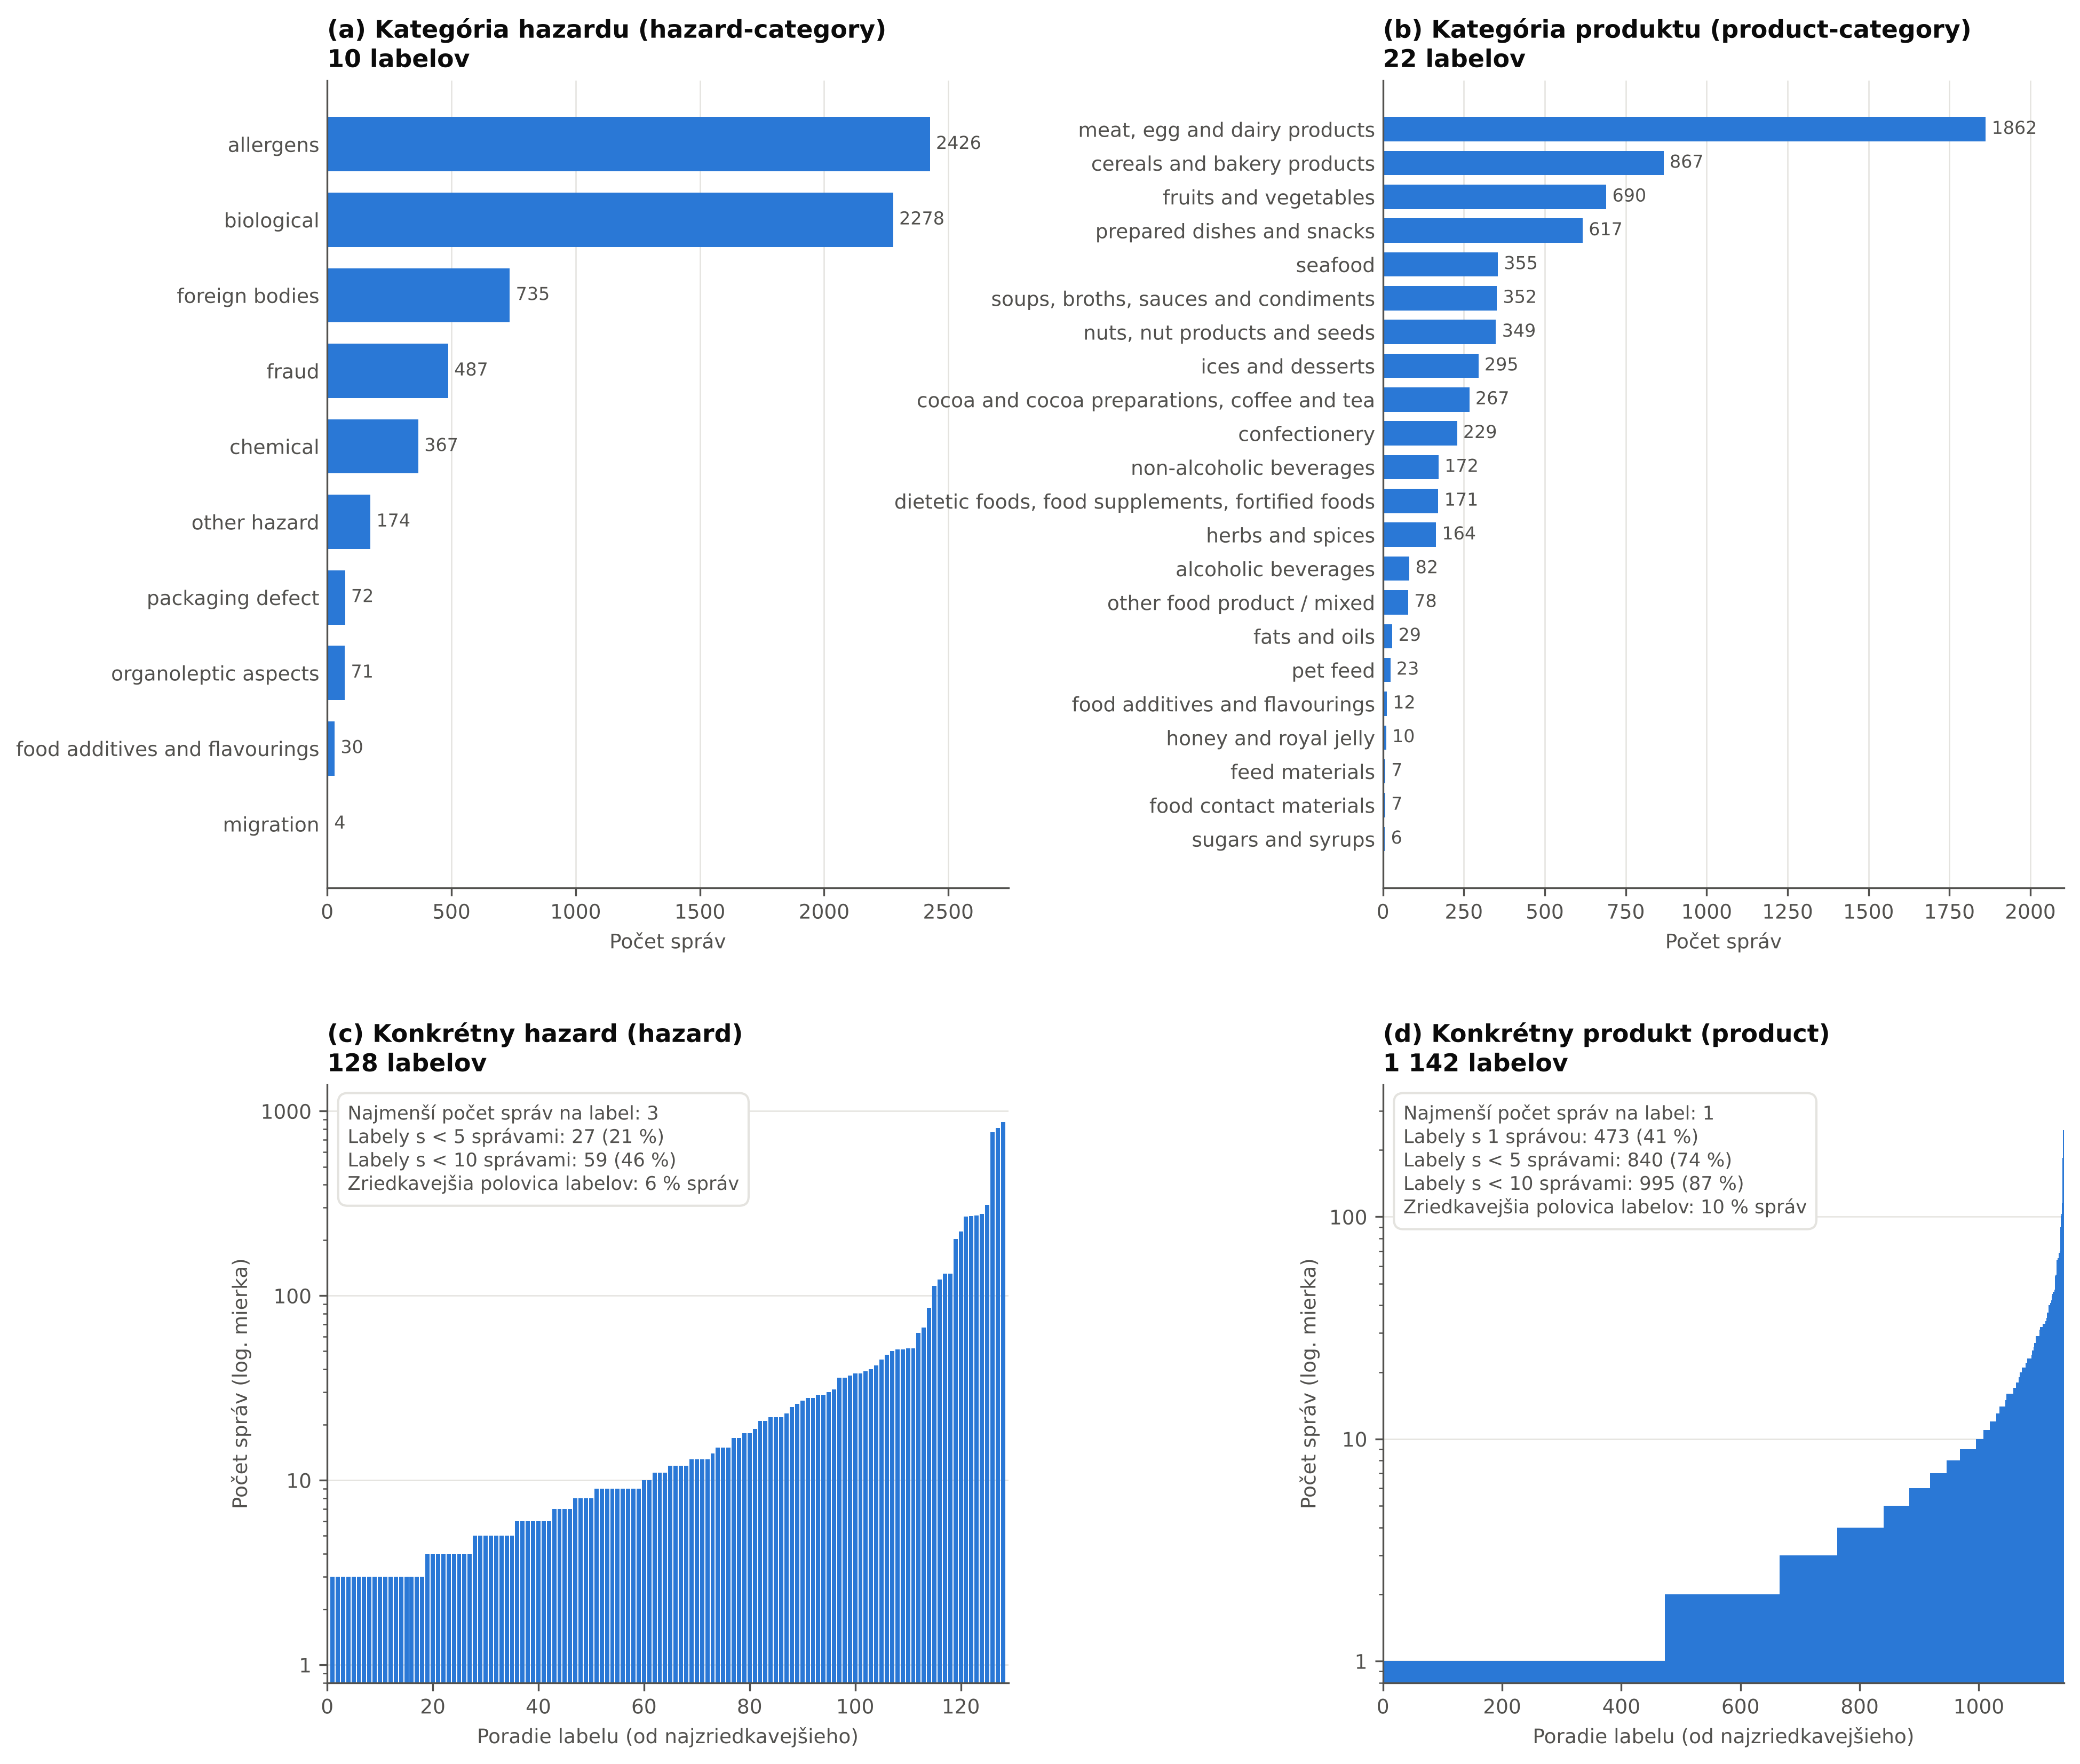
\includegraphics[width=0.95\textwidth]{figures/dataset_distribution.png}
    \caption{Distribúcie cieľových atribút v poskytnutom datasete.}
    \label{fig:dataset_distribution}
\end{figure}

\begin{comment}
\subsection{Prehľad riešení dosahujúcich najlepšie výsledky}

The most important literature source for this project is the official SemEval-2025 Task 9 report \cite{randl-etal-2025-semeval}. Included within this report is a section highlighting the 4 best performing submitted solutions with references to their individual papers. The following subsections will briefly describe the methods used in the solutions. This information will then be used in order to formulate an appropriate baseline for this project.

\subsubsection{SRCB (Ricoh Software Research Center (Beijing)) \cite{zhang-etal-2025-srcb}} 

For data pre-processing the system first concatenates the \textit{title} and \textit{text} (which were the only input features used) into a single text format, which is then cleaned to remove various text artifacts such as line breaks, spaces, duplicate lines etc. The resulting texts are then truncated to a maximum token length in order to be used for inputs for the two modules the system employs (512 and 1024 respectively).   

For data augmentation a method involving an LLM was used (specifically the Qwen2.5-72B-Instruct), where the LLM was instructed to create a new sample based on the meaning and label of a target sample from a rare (fewer than 50 occurrences in the training data) class and writing style and format of a randomly selected sample.

The actual system used two primary modules : a candidate recall module and an LLM prediction module. The role of the candidate recall module is to help narrow the set of possible output labels before the more computationally expensive LLM prediction. This module uses a one-vs-all approach, constructing a binary classifier for each label on top of a BERT architecture. This approach was chosen due to the fact that the authors experimented with the RoBERTa-base model and found that while the score for classification was rather poor, the recall score achieved a value over 95\% indicating that the correct label would almost always be found in the candidate labels outputted by the BERT model. In the final submission this module was built using the RoBERTa-base and DeBERTaV3-base models.

The LLM prediction module is more complex, involving two LLMs : a fine tuned target LLM and a frozen reference LLM that is used to pre-compute embeddings of all labels before training. These embeddings are then used as external background knowledge together with the output of the target LLM (which uses the formatted text body and the reduced label set from the previous module) inside of a multi-head attention module, the outputs of which are then used to generate the final label as text. For both roles the authors used the Qwen2.5-14B-Base model. The final submission from this team combined several variants of this pipeline with majority voting, however the exact details of the variants used are not described in the report. 

This solution ranked third for ST1 and first(!) for ST2, with two separate but architecturally same pipelines for each subtask. 

\begin{figure}
    \centering
    \includegraphics[width=0.95\textwidth]{figures/SRCB_Figure2_LLM_Prediction_Module.png}
    \caption{Architecture of the LLM prediction module (taken directly from \cite{zhang-etal-2025-srcb}).}
    \label{fig:srcb_llm_prediction_module}
\end{figure}
\end{comment}

\subsection{Prehľad riešení dosahujúcich najlepšie výsledky}

Najdôležitejším literárnym zdrojom pre tento projekt je oficiálna správa k SemEval-2025 Task 9 \cite{randl-etal-2025-semeval}. Táto správa obsahuje sekciu, v ktorej sú vyzdvihnuté 4 najlepšie odovzdané riešenia spolu s odkazmi na ich jednotlivé články. V nasledujúcich podkapitolách budú stručne opísané metódy použité v týchto riešeniach. Tieto informácie budú následne použité na sformulovanie vhodného baseline riešenia pre tento projekt.

\subsubsection{SRCB (Ricoh Software Research Center (Beijing)) \cite{zhang-etal-2025-srcb}}

V rámci predspracovania dát systém najprv spojí atribúty \textit{title} a \textit{text} (ktoré boli jedinými použitými vstupnými atribútmi) do jedného textu, ktorý je následne vyčistený od rôznych textových artefaktov, ako sú zalomenia riadkov, nadbytočné medzery, duplicitné riadky a pod. Výsledné texty sú následne skrátené na maximálnu dĺžku v tokenoch, aby mohli byť použité ako vstupy pre dva moduly, ktoré systém využíva (512, resp. 1024 tokenov).

Na augmentáciu dát bola použitá metóda využívajúca LLM (konkrétne model Qwen2.5-72B-Instruct), pričom LLM bol inštruovaný vytvoriť novú vzorku, ktorá preberá význam a označenie cieľovej vzorky zo zriedkavej triedy (menej ako 50 výskytov v trénovacích dátach) a štýl písania a formát náhodne vybranej vzorky.

Samotný systém využíval dva hlavné moduly: modul na výber kandidátov (candidate recall module) a modul predikcie pomocou LLM (LLM prediction module). Úlohou modulu na výber kandidátov je zúžiť množinu možných výstupných označení pred výpočtovo náročnejšou predikciou pomocou LLM. Tento modul využíva prístup one-vs-all, pričom pre každé označenie je zostrojený binárny klasifikátor nad architektúrou BERT. Tento prístup bol zvolený, pretože autori experimentovali s modelom RoBERTa-base a zistili, že hoci skóre klasifikácie bolo pomerne slabé, hodnota recall presahovala 95~\%, čo naznačuje, že správne označenie sa takmer vždy nachádza medzi kandidátskymi označeniami na výstupe modelu BERT. Vo finálnom odovzdanom riešení bol tento modul zostavený s použitím modelov RoBERTa-base a DeBERTaV3-base.

Modul predikcie pomocou LLM je zložitejší a zahŕňa dva LLM: doladený (fine-tuned) cieľový LLM a zmrazený referenčný LLM, ktorý je použitý na predvýpočet embeddingov všetkých označení ešte pred trénovaním. Tieto embeddingy sú následne použité ako externé doplnkové znalosti spolu s výstupom cieľového LLM (ktorý na vstupe dostáva naformátovaný text a zúženú množinu označení z predchádzajúceho modulu) v module multi-head attention, ktorého výstupy sú následne použité na vygenerovanie výsledného označenia vo forme textu. Pre obe roly autori použili model Qwen2.5-14B-Base. Finálne odovzdané riešenie tohto tímu kombinovalo niekoľko variantov tejto pipeline pomocou väčšinového hlasovania, avšak presné detaily použitých variantov nie sú v správe opísané.

Toto riešenie sa umiestnilo na treťom mieste v ST1 a na prvom(!) mieste v ST2, pričom pre každú podúlohu bola použitá samostatná, no architektonicky rovnaká pipeline.

\begin{figure}
    \centering
    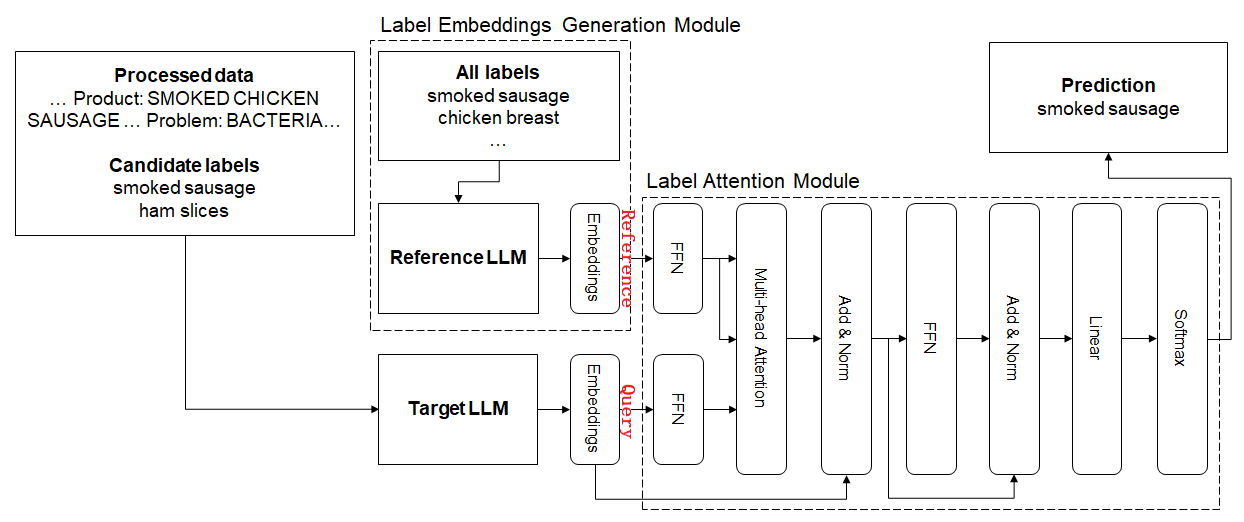
\includegraphics[width=0.95\textwidth]{figures/srcb_prediction_module.png}
    \caption{Architektúra modulu predikcie pomocou LLM (prevzaté priamo z \cite{zhang-etal-2025-srcb}).}
    \label{fig:srcb_llm_prediction_module}
\end{figure}

\begin{comment}
\subsubsection{Anastasia \cite{le-etal-2025-anastasia}}

This system uses an ensemble approach focusing exclusively on ST1. For data pre-processing the system first (seemingly) concatenates all of the provided input features.Standard text cleaning techniques are then applied to remove artifacts similar to the SRCB solution. Various degrees of data augmentation (including none) are then employed to create three separate datasets that are used by the system's modules. The resulting entries of the datasets are then divided into sentence-based chunks of various sizes in order to be used as inputs for the various models inside the modules, concretely sizes of 512, 768, 1024 and 1280 token chunks.

The three datasets used were:

\begin{enumerate}
    \item \textit{Original} -- features no synthetic samples, only oversampling and undersampling techniques, which were employed in order to help balance out the dataset
    
    \item \textit{Light Augmentation} -- features data augmentation, specifically the creation of synthetic samples of underpopulated classes (the exact method of the creation of these samples is not detailed in the article)
    
    \item \textit{Heavy Augmentation} -- same as Light Augmentation, however with larger quantities of synthetic samples and extra processing steps
\end{enumerate}

For the \textit{Heavy Augmentation} additional processing techniques were used such as HTML tag removal with the help of BeautifulSoup \cite{pant2024web} and the translation of the non-English entries included in the original data, helping to further increase the consistency and size of this variation of the dataset. 

As previously mentioned this solution uses three system modules, with two of these modules focusing on a single-task prediction (product category and hazard category respectively) and the third one on a multi-task prediction of both target features. The single-task modules in total feature 24 models (12 configurations for hazard and product category respectively) based on the combination of the light/heavy dataset, DeBERTa-v3-large/RoBERTa-large model, and the 512/768/1024/1280 token chunk size. For the multitask module only the DeBERTa-v3-large model was used with a token chunk size of 512, using the \textit{Original} dataset. For the exact combinations used see Figure~\ref{fig:anastasia_models}.

\begin{figure}
    \centering
    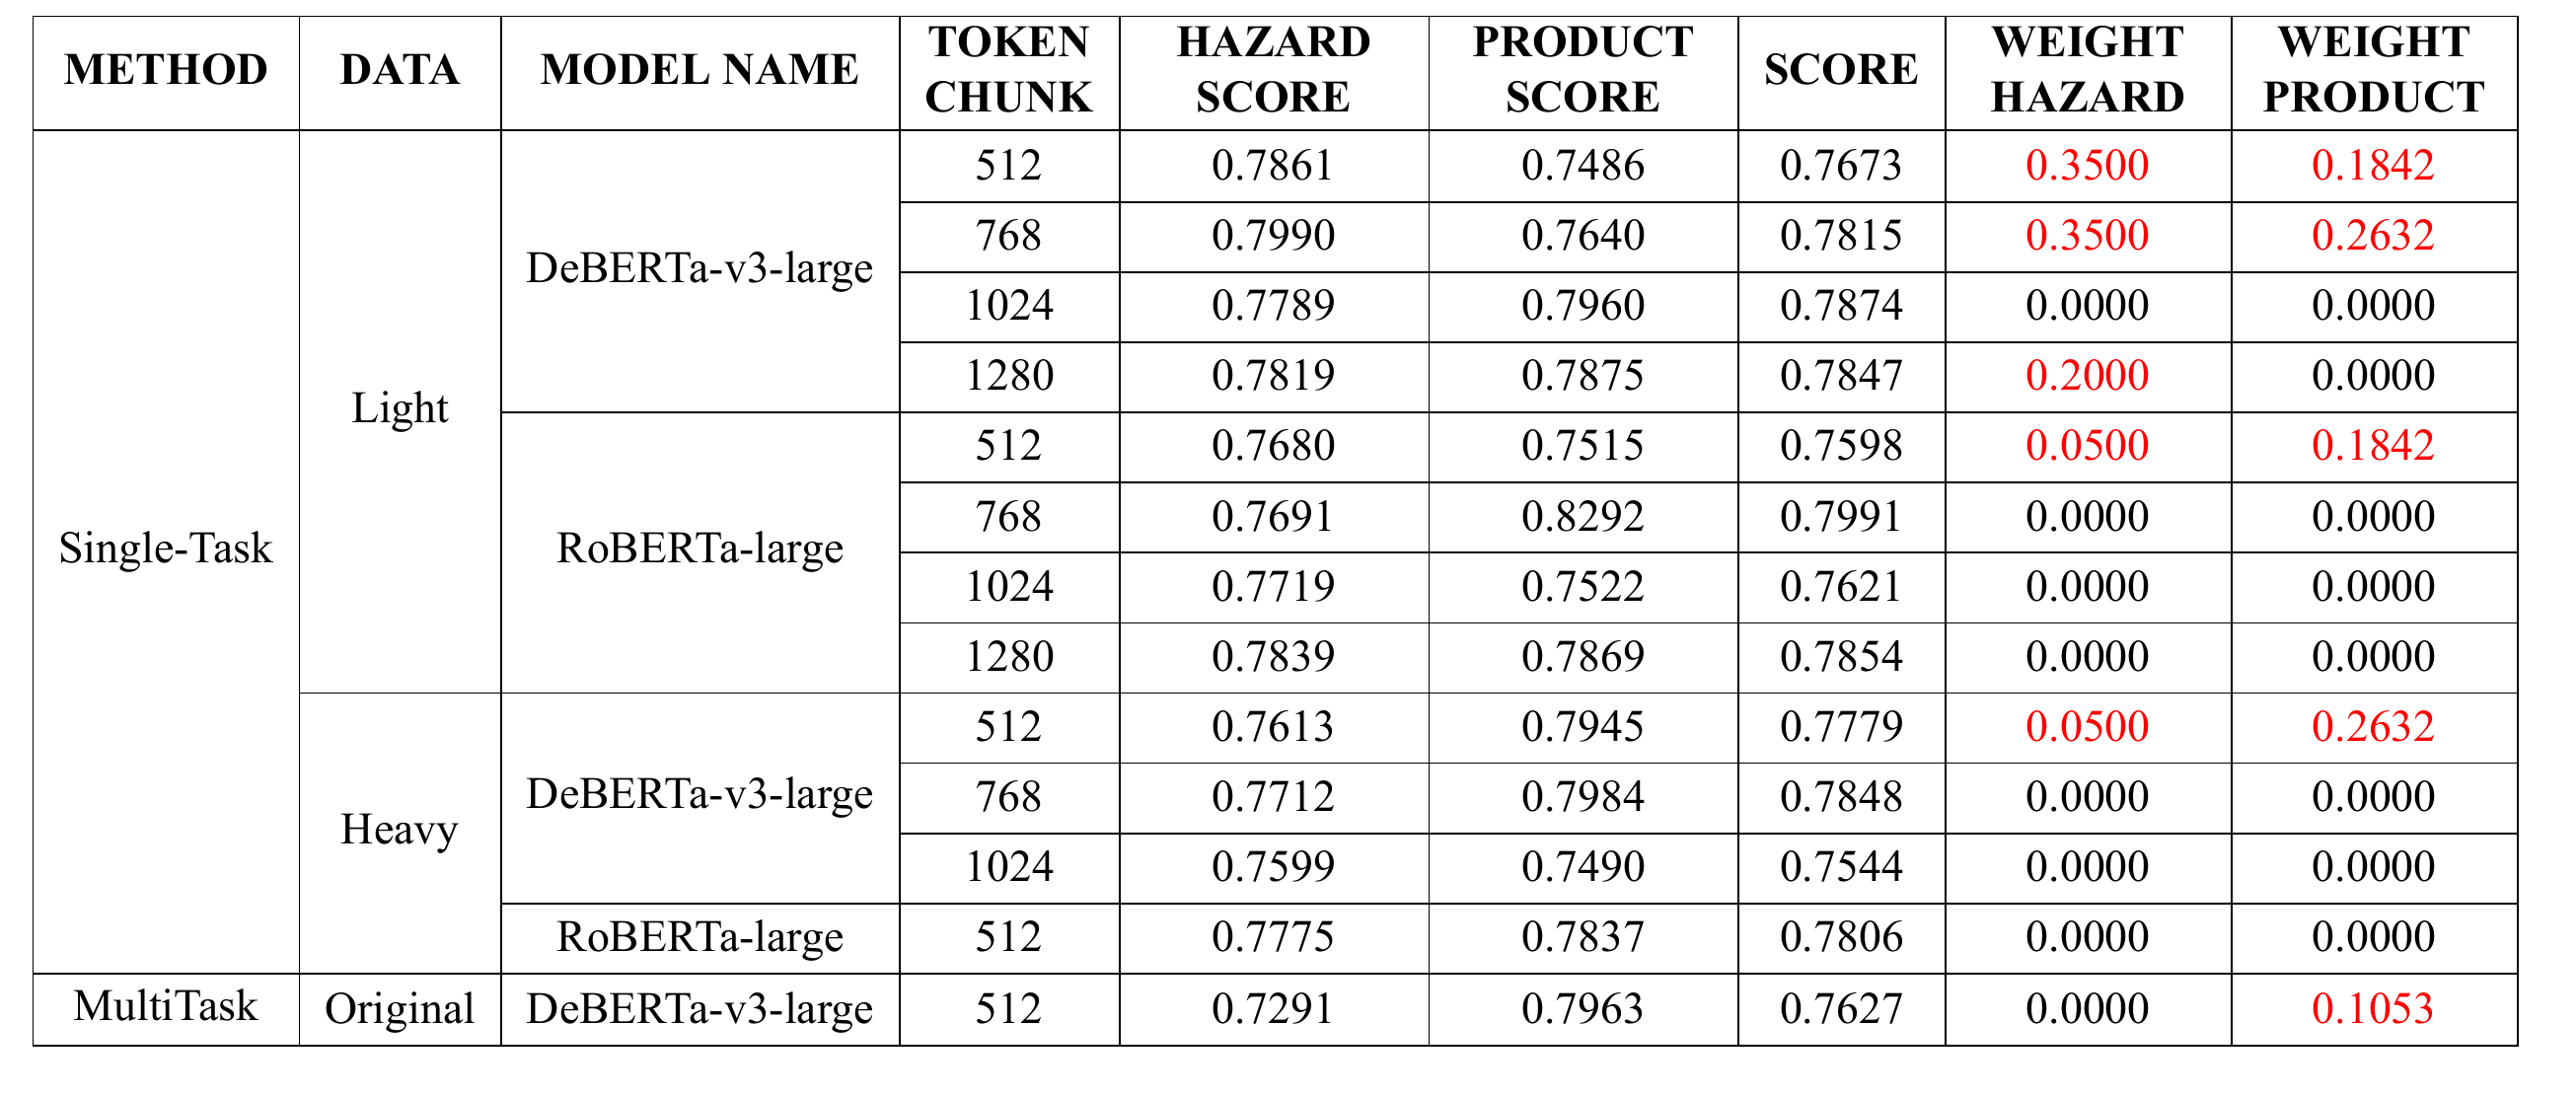
\includegraphics[width=0.95\textwidth]{figures/anastasia_models.png}
    \caption{Exact combinations of models used as part of the solution, each single-task row represents two models (one for the hazard and product category respectively) also including the final weights used in soft-voting (taken directly from \cite{le-etal-2025-anastasia}).}
    \label{fig:anastasia_models}
\end{figure}

To obtain the final prediction, weighted soft voting is applied separately for the hazard and product category, the exact weights of which were obtained with the help of a grid search technique. Another aspect that is important to highlight is the use of the loss function: Focal loss \cite{lin2017focal}. This loss function (see Equation~\eqref{eq:focal_loss}) is designed to reduce the impact of easy-to-classify samples  while prioritizing the harder ones, further helping to reduce the impact of the imbalanced dataset. This function was used in the fine-tuning process of all the models.

\begin{equation}
  \mathcal{L}_{FL}(p_t) = -\alpha_t (1 - p_t)^{\gamma} \log(p_t)
  \label{eq:focal_loss}
\end{equation}

This solution ranked first(!) for ST1. However, the authors acknowledge that they submitted multiple test runs, violating SemEval's single-submission rule, which may have given them an advantage.
\end{comment}

\subsubsection{Anastasia \cite{le-etal-2025-anastasia}}

Tento systém využíva ensemble prístup a zameriava sa výlučne na ST1. V rámci predspracovania dát systém najprv (zrejme) spojí všetky poskytnuté vstupné atribúty. Následne sú aplikované štandardné techniky čistenia textu na odstránenie artefaktov, podobne ako v riešení SRCB. Potom je použitá augmentácia dát v rôznej miere (vrátane žiadnej) na vytvorenie troch samostatných datasetov, ktoré sú využívané modulmi systému. Záznamy výsledných datasetov sú následne rozdelené na úseky (chunky) založené na vetách s rôznou veľkosťou, aby mohli byť použité ako vstupy pre jednotlivé modely v moduloch, konkrétne s veľkosťou 512, 768, 1024 a 1280 tokenov.

Použité boli tieto tri datasety:

\begin{enumerate}
    \item \textit{Original} -- neobsahuje syntetické vzorky, iba techniky oversamplingu a undersamplingu, ktoré boli použité na vyváženie datasetu
    
    \item \textit{Light Augmentation} -- obsahuje augmentované dáta, konkrétne syntetické vzorky málo zastúpených tried (presná metóda vytvorenia týchto vzoriek nie je v článku opísaná)
    
    \item \textit{Heavy Augmentation} -- rovnaký ako Light Augmentation, avšak s väčším množstvom syntetických vzoriek a dodatočnými krokmi spracovania
\end{enumerate}

Pri datasete \textit{Heavy Augmentation} boli použité dodatočné techniky spracovania, ako napríklad odstránenie HTML tagov pomocou knižnice BeautifulSoup \cite{pant2024web} a preklad neanglických záznamov obsiahnutých v pôvodných dátach, čo pomohlo ďalej zvýšiť konzistenciu a veľkosť tejto verzie datasetu.

Ako už bolo spomenuté, toto riešenie využíva tri moduly, pričom dva z nich sa zameriavajú na predikciu jedného cieľového atribútu (single-task), konkrétne kategórie produktu, resp. kategórie hazardu, a tretí na súčasnú predikciu oboch cieľových atribútov (multi-task). Single-task moduly spolu obsahujú 24 modelov (12 konfigurácií pre kategóriu hazardu a 12 pre kategóriu produktu), ktoré vychádzajú z kombinácie datasetu light/heavy, modelu DeBERTa-v3-large/RoBERTa-large a veľkosti chunku 512/768/1024/1280 tokenov. Pre multi-task modul bol použitý iba model DeBERTa-v3-large s veľkosťou chunku 512 tokenov a datasetom \textit{Original}. Pre použité kombinácie viď obrázok~\ref{fig:anastasia_models}.

\begin{figure}
    \centering
    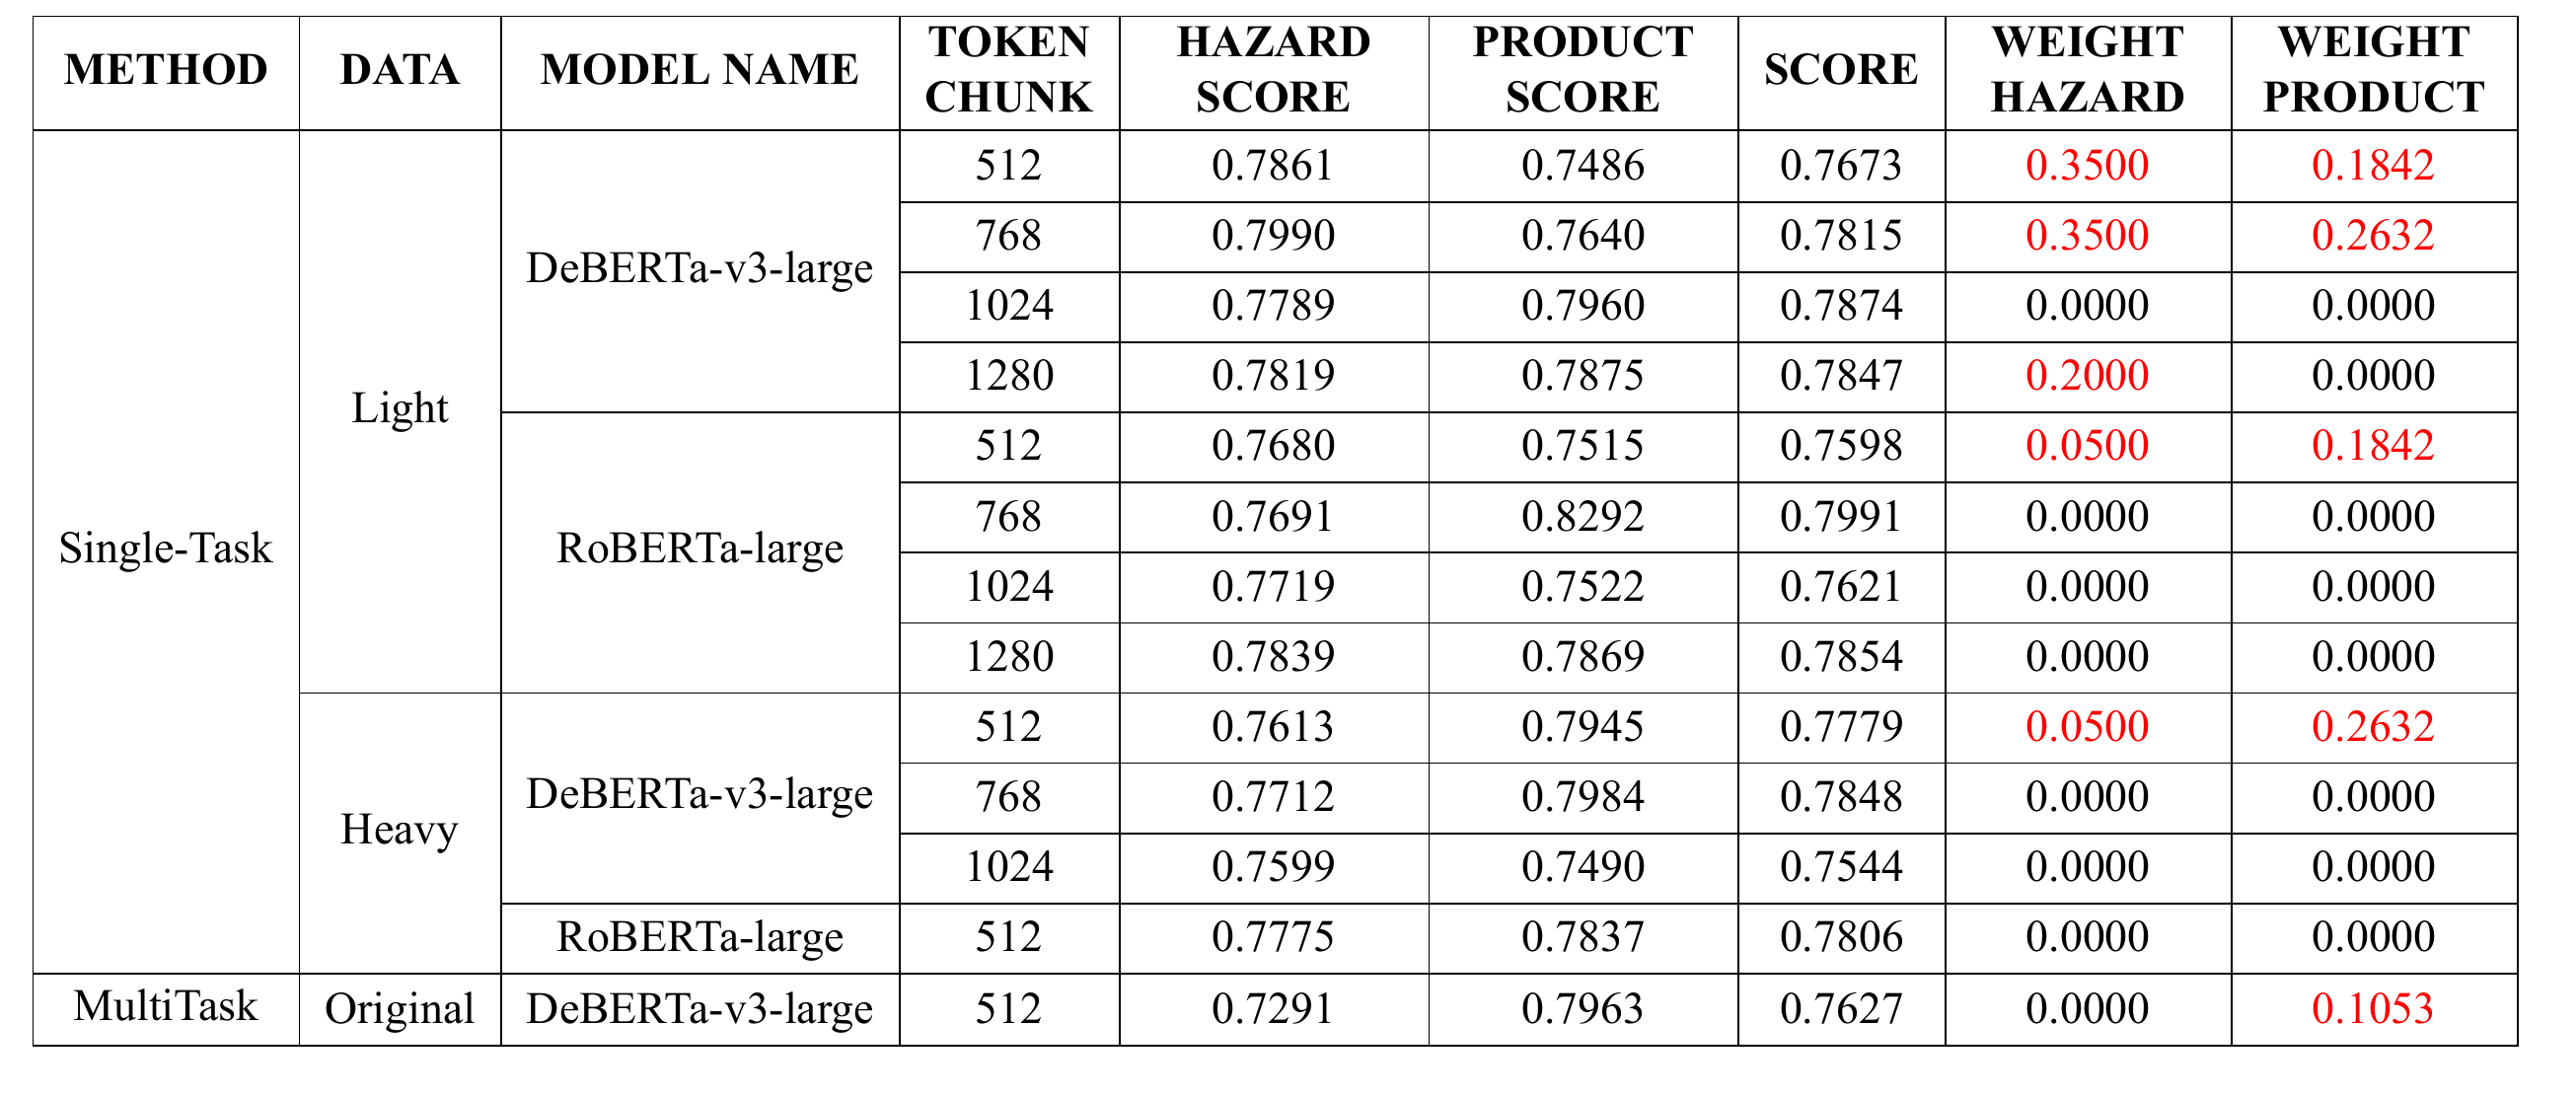
\includegraphics[width=0.95\textwidth]{figures/anastasia_models.png}
    \caption{Presné kombinácie modelov použitých v riešení. Každý single-task riadok predstavuje dva modely (jeden pre kategóriu hazardu a jeden pre kategóriu produktu) a obsahuje aj výsledné váhy použité pri mäkkom hlasovaní (prevzaté priamo z \cite{le-etal-2025-anastasia}).}
    \label{fig:anastasia_models}
\end{figure}

Na získanie finálnej predikcie je samostatne pre kategóriu hazardu a kategóriu produktu použité vážené mäkké hlasovanie (weighted soft voting), pričom presné váhy boli získané pomocou techniky grid search. Ďalším dôležitým aspektom, ktorý je potrebné zdôrazniť, je použitie loss funkcie Focal loss \cite{lin2017focal}. Táto loss funkcia (viď rovnicu~\eqref{eq:focal_loss}) je navrhnutá tak, aby znižovala vplyv ľahko klasifikovateľných vzoriek a uprednostňovala tie ťažšie, čo ďalej pomáha zmierniť vplyv nevyváženosti datasetu. Táto funkcia bola použitá pri doladení (fine-tuning) všetkých modelov.

\begin{equation}
  \mathcal{L}_{FL}(p_t) = -\alpha_t (1 - p_t)^{\gamma} \log(p_t)
  \label{eq:focal_loss}
\end{equation}

Toto riešenie sa umiestnilo na prvom(!) mieste v ST1. Autori však uvádzajú, že odovzdali viacero testovacích behov, čím porušili pravidlo SemEval o jedinom odovzdaní, čo im mohlo poskytnúť výhodu.

\begin{comment}
\subsubsection{MyMy \cite{phan-chiang-2025-mymy}}

This system is notable due to its focus on creating robust synthetic samples as part of data augmentation. For pre-processing the system does not seem to employ any sort of standard text cleaning procedure, only stating that the solution utilizes all provided input features.

The most important component of this system is the robust data augmentation pipeline, which utilizes a RAG technique in order to create rich synthetic samples to add to the dataset based on contextual documents retrieved from PubMed, a publicly accessible database for biomedical literature. First the original samples are fed to LLMs which are prompted with creating a short search query for each sample. This is done to help increase the effectiveness of document retrieval from PubMed API, which is otherwise prone to failure with complex queries. Based on the query the relevant documents are then retrieved from the PubMed API, and subsequently converted into dense vectors and stored in a Chroma vector database for efficient searching by cosine similarity. Next, the top-K (the value of this parameter is not stated in the report) most similar documents to the original text are inserted (together with original text itself) into the prompt format of the following step.

The resulting prompts are then passed to LLMs, which are instructed (as part of the prompt) with creating a synthetic sample by paraphrasing the original text while using the provided context. As a final step of data augmentation the resulting texts are then passed to LLMs, which are prompted with grading the quality of the created sample with a score from 0 to 5, based on relevance and accuracy against the included context. Only samples that receive a score of 4 or 5 are added to the resulting dataset. Roughly 60\,000 augmented samples passed this filtering step and were added to the dataset against the 5\,082 original samples, helping greatly in increasing the size of the dataset. The LLMs used in this augmentation pipeline were GPT-3.5 Turbo, Gemini Flash 2.0, Llama 3.1 8B, and Mixtral 8x7B. 

Compared to the data augmentation pipeline, the prediction pipeline is rather simple utilizing Gemini Flash 2.0, PubMedBERT and ModernBERT fine-tuned on the enriched dataset. The predicted labels are then computed using an ensemble strategy, specifically by averaging class probabilities of each of the models for each sub-task.

This solution ranked second on both ST1 and ST2, demonstrating itself as the most balanced of the highlighted solutions.  

\begin{figure}
    \centering
    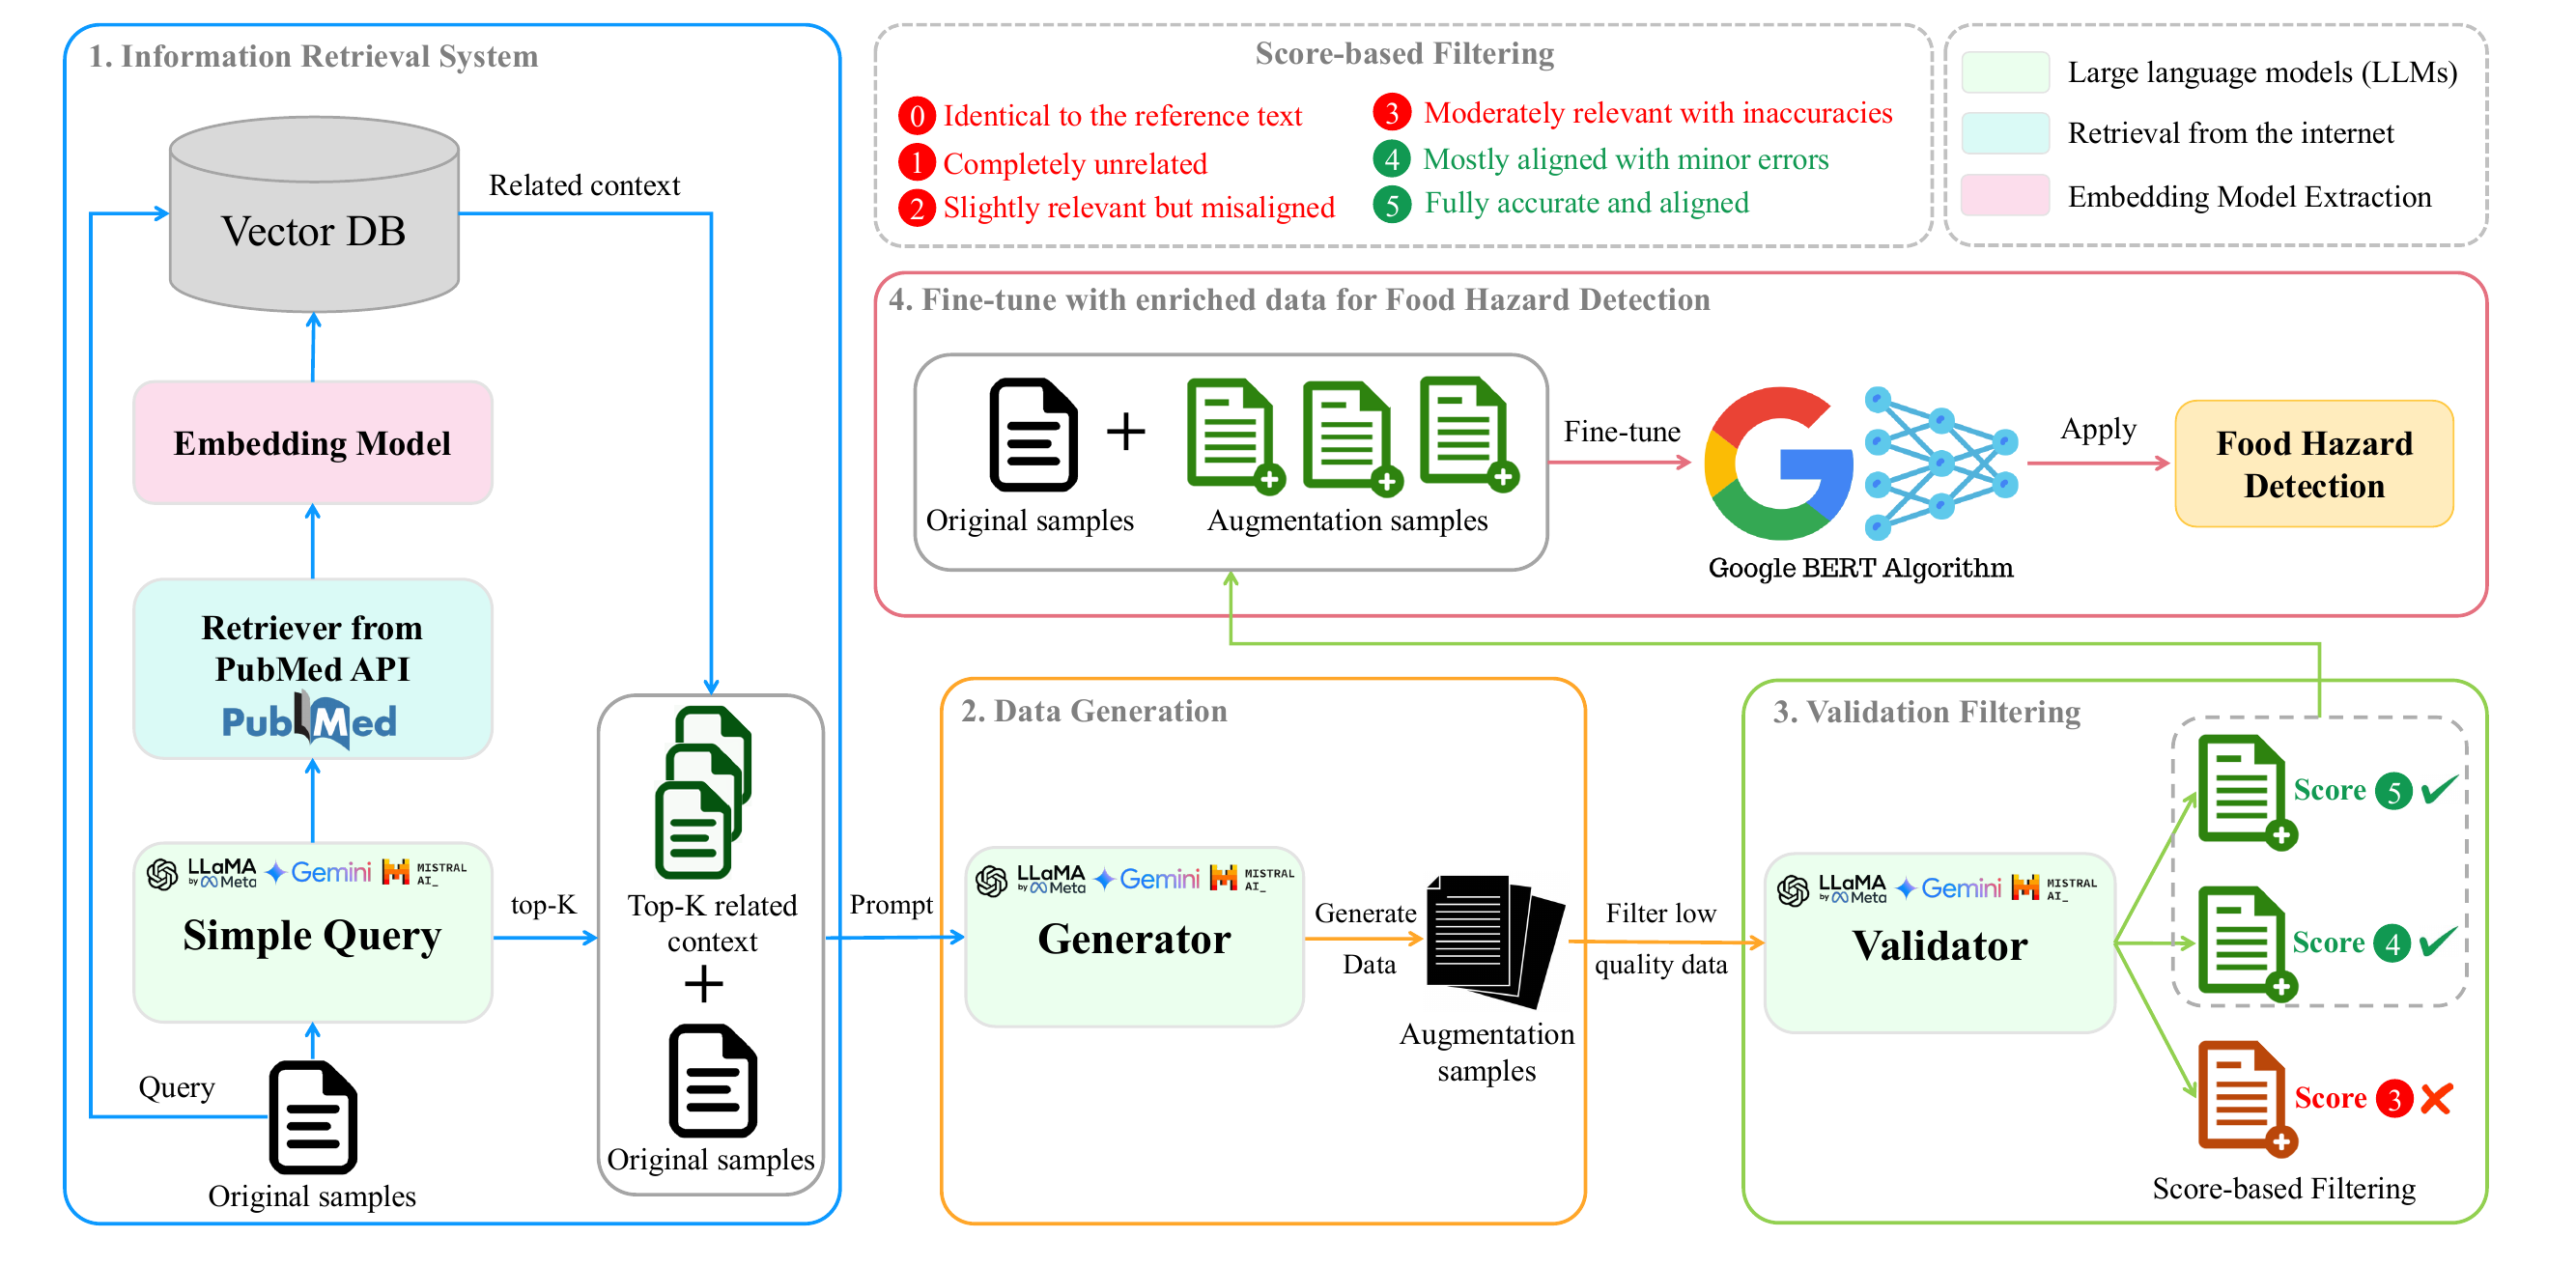
\includegraphics[width=0.95\textwidth]{figures/mymy_architecture.png}
    \caption{Data augmentation pipeline and system architecture used in the MyMy solution, Google BERT is only used as a visualization, the models fine-tuned as a part of the solution were Gemini Flash 2.0, PubMedBERT
    and ModernBERT (taken directly from \cite{phan-chiang-2025-mymy}).}
    \label{fig:mymy_architecture}
\end{figure}
\end{comment}

\subsubsection{MyMy \cite{phan-chiang-2025-mymy}}

Tento systém je pozoruhodný vďaka zameraniu na tvorbu robustných syntetických vzoriek v rámci augmentácie dát. V rámci predspracovania systém zrejme nevyužíva žiadny štandardný postup čistenia textu, pričom autori uvádzajú iba to, že riešenie využíva všetky poskytnuté vstupné atribúty.

Najdôležitejšou súčasťou tohto systému je robustná pipeline na augmentáciu dát, ktorá využíva techniku RAG na tvorbu obsahovo bohatých syntetických vzoriek pridávaných do datasetu na základe kontextových dokumentov získaných z PubMed, verejne dostupnej databázy biomedicínskej literatúry. Najprv sú pôvodné vzorky predané LLM, ktoré sú inštruované vytvoriť pre každú vzorku krátky vyhľadávací dopyt. Účelom tohto kroku je zvýšiť efektivitu získavania dokumentov z PubMed API, ktoré je inak pri zložitých dopytoch náchylné na zlyhanie. Na základe dopytu sú následne z PubMed API získané relevantné dokumenty, ktoré sú potom prevedené na dense vektory a uložené vo vektorovej databáze Chroma na efektívne vyhľadávanie pomocou kosínusovej podobnosti. Ďalej je top-K dokumentov najpodobnejších pôvodnému textu (hodnota tohto parametra nie je v správe uvedená) vložených (spolu so samotným pôvodným textom) do promptu nasledujúceho kroku.

Výsledné prompty sú následne predané LLM, ktoré sú (v rámci promptu) inštruované vytvoriť syntetickú vzorku parafrázovaním pôvodného textu s využitím poskytnutého kontextu. V poslednom kroku augmentácie dát sú výsledné texty predané LLM, ktoré sú inštruované ohodnotiť kvalitu vytvorenej vzorky od 0 do 5 na základe relevantnosti a presnosti vzhľadom na priložený kontext. Do výsledného datasetu sú pridané iba vzorky, ktoré získali skóre 4 alebo 5. Týmto filtrovaním úspešne prešlo približne 60\,000 augmentovaných vzoriek, ktoré boli pridané do datasetu oproti 5\,082 pôvodným vzorkám, čo výrazne pomohlo zväčšiť veľkosť datasetu. V tejto augmentačnej pipeline boli použité modely GPT-3.5 Turbo, Gemini Flash 2.0, Llama 3.1 8B a Mixtral 8x7B.

V porovnaní s pipeline na augmentáciu dát je predikčná pipeline pomerne jednoduchá a využíva modely Gemini Flash 2.0, PubMedBERT a ModernBERT doladené na obohatenom datasete. Predikované označenia sú následne vypočítané pomocou ensemble stratégie, konkrétne spriemerovaním pravdepodobností tried jednotlivých modelov pre každú podúlohu.

Toto riešenie sa umiestnilo na druhom mieste v ST1 aj ST2, čím sa ukázalo ako najvyváženejšie zo spomenutých riešení.

\begin{figure}
    \centering
    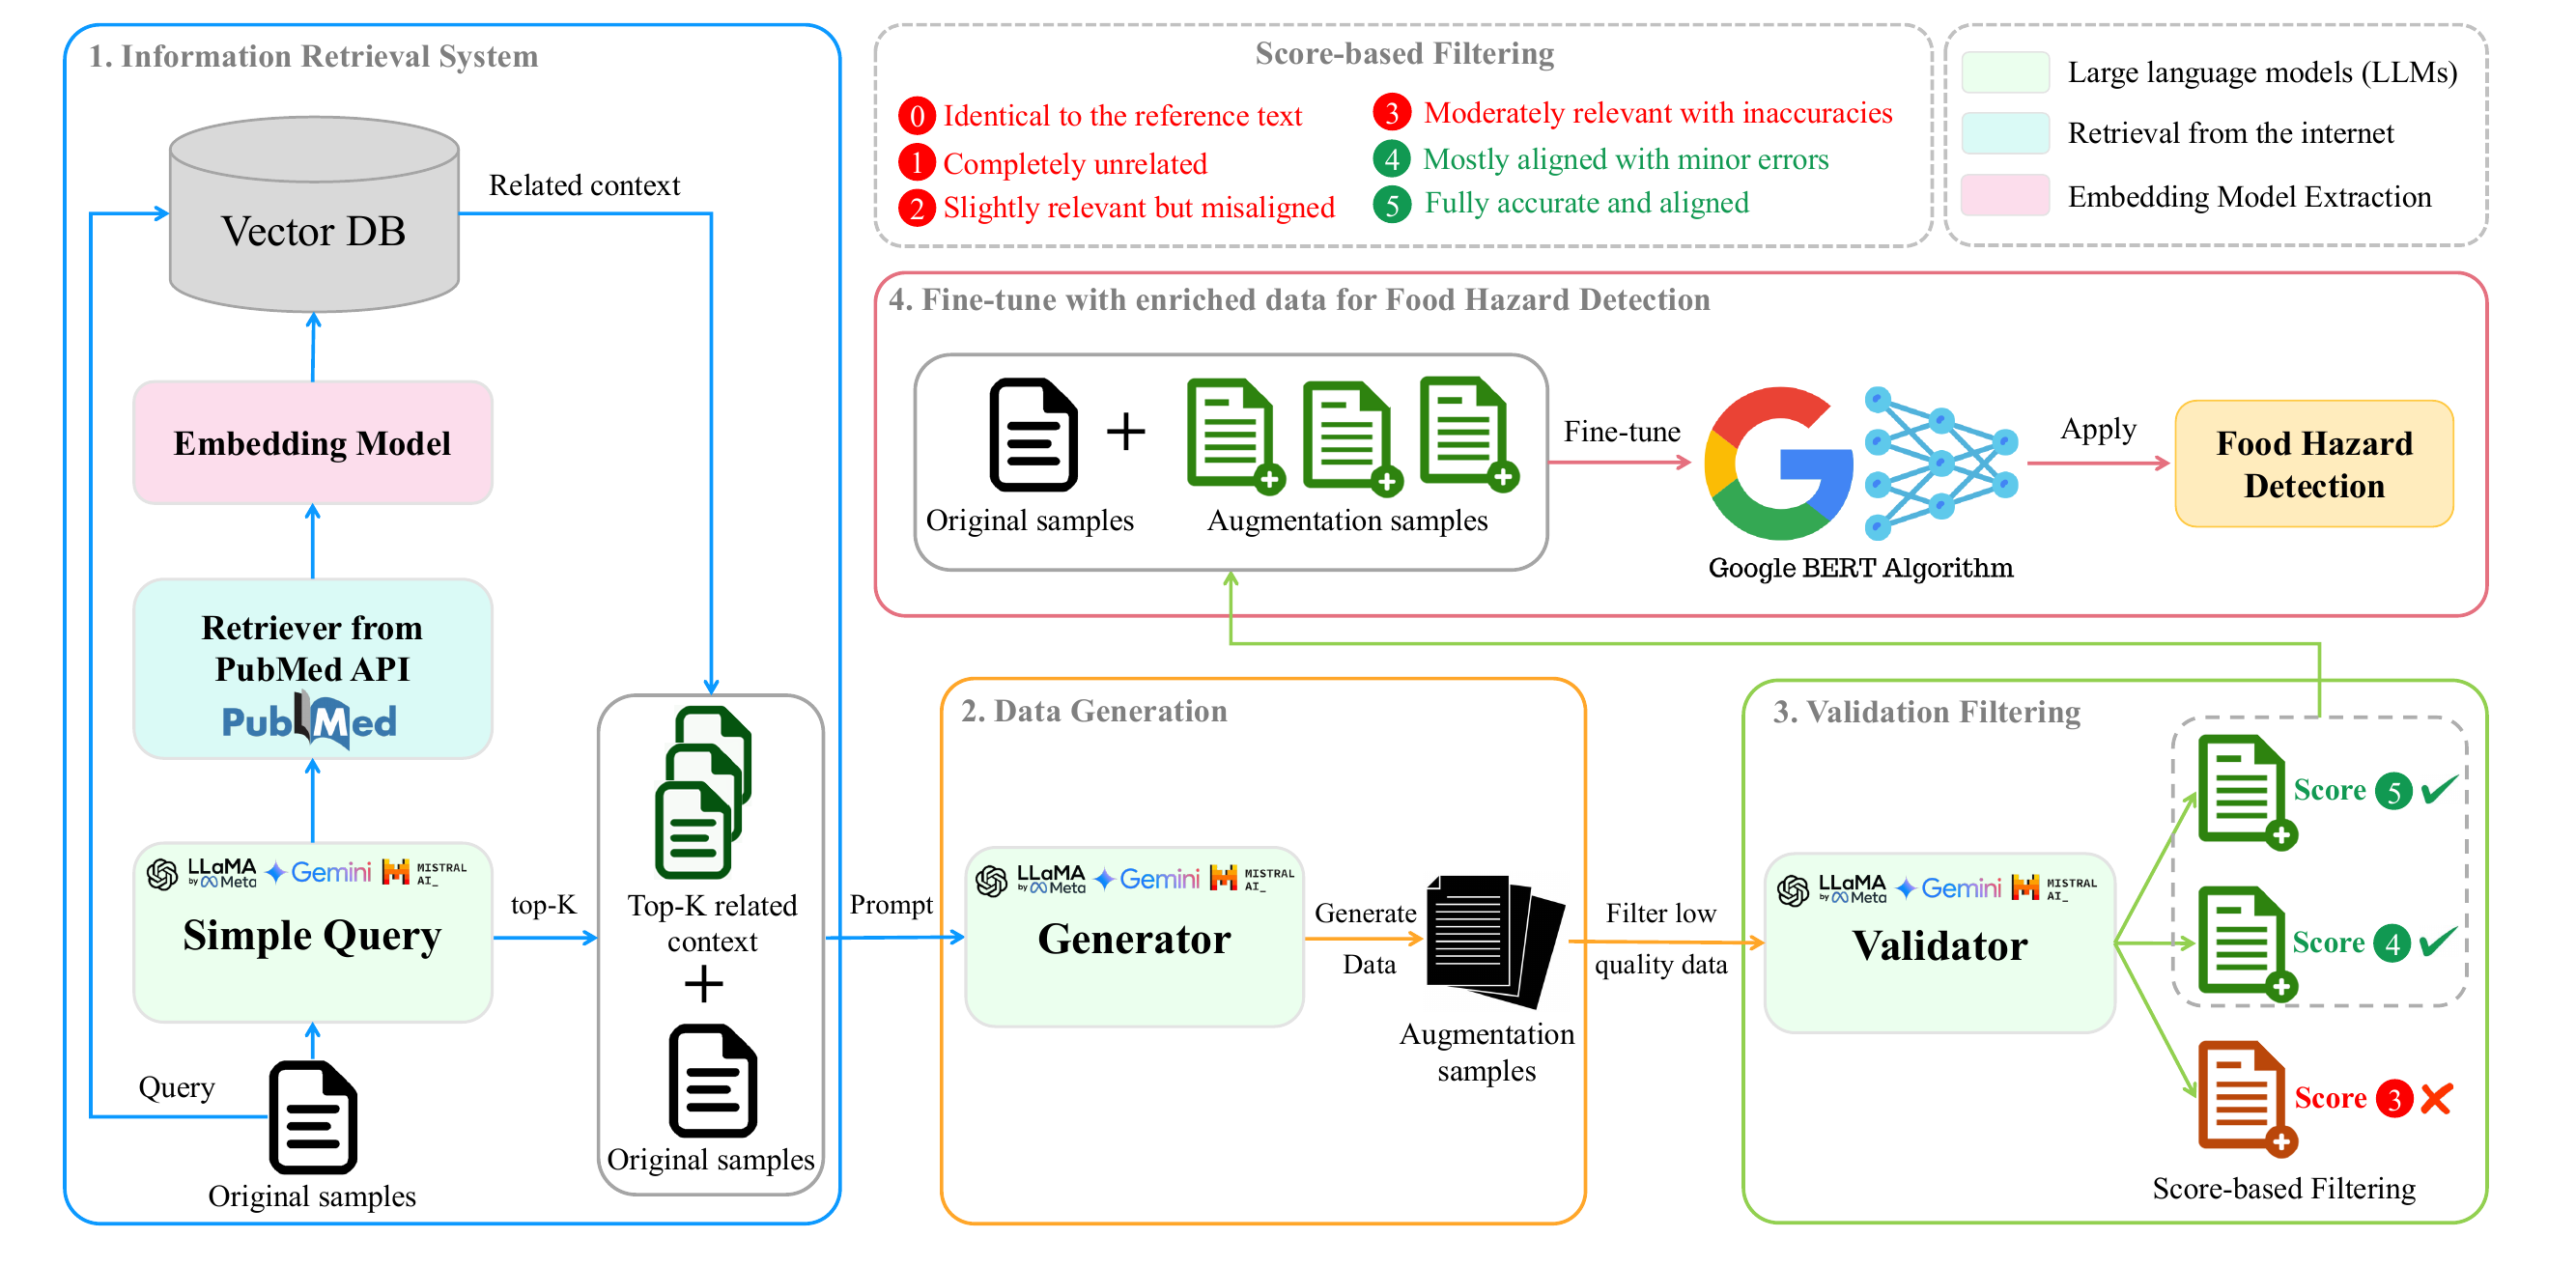
\includegraphics[width=0.95\textwidth]{figures/mymy_architecture.png}
    \caption{Pipeline na augmentáciu dát a architektúra systému použité v riešení MyMy. Google BERT slúži iba na ilustráciu, modely doladené v rámci riešenia boli Gemini Flash 2.0, PubMedBERT a ModernBERT (prevzaté priamo z \cite{phan-chiang-2025-mymy}).}
    \label{fig:mymy_architecture}
\end{figure}

\begin{comment}
\subsubsection{PATeam \cite{wan-etal-2025-pateam}}

This system is notable for its use of a single generative LLM that solves both sub-tasks jointly in a multi-turn dialogue format, combined with a bagging ensemble. For pre-processing, the authors use regular expressions to remove unwanted web artifacts such as hyperlinks, HTML formatting and e-mail addresses. Only the \textit{title} and \textit{text} input features are used.

For data augmentation, an LLM is prompted to generate a concise summary of each cleaned text, which is then concatenated with the original text. Unlike the other highlighted solutions, this does not create new samples but enriches the existing ones; according to the authors, the summaries help standardise the noisy texts and highlight the information relevant to the product and hazard labels. The LLM used for summarisation is not named in the text, although the system overview (Figure~\ref{fig:pateam_overview}) indicates Qwen2.5-72B. To address the class imbalance, the enriched dataset is then oversampled so that every class contains at least five samples, a threshold the authors found to work best on the validation set.

The prediction itself is done by Phi-4, fine-tuned with LoRA \cite{hu2021lora}, which formulates the two sub-tasks as a two-round dialogue. In the first round, the model receives the title, the cleaned text and the generated summary and predicts the hazard and product category (ST1). In the second round, these predictions are added to the prompt and the model is asked to infer the more specific hazard and product (ST2). This way, the coarse-grained prediction guides the fine-grained one. For the ensemble, a bagging approach \cite{breiman1996bagging} is used: five subsets of the training data are sampled with replacement, a separate Phi-4 model is fine-tuned on each of them, and the final prediction is obtained by voting between the five models (the exact voting scheme is not specified).

This solution ranked fourth in ST1 and third in ST2.

\begin{figure}
    \centering
    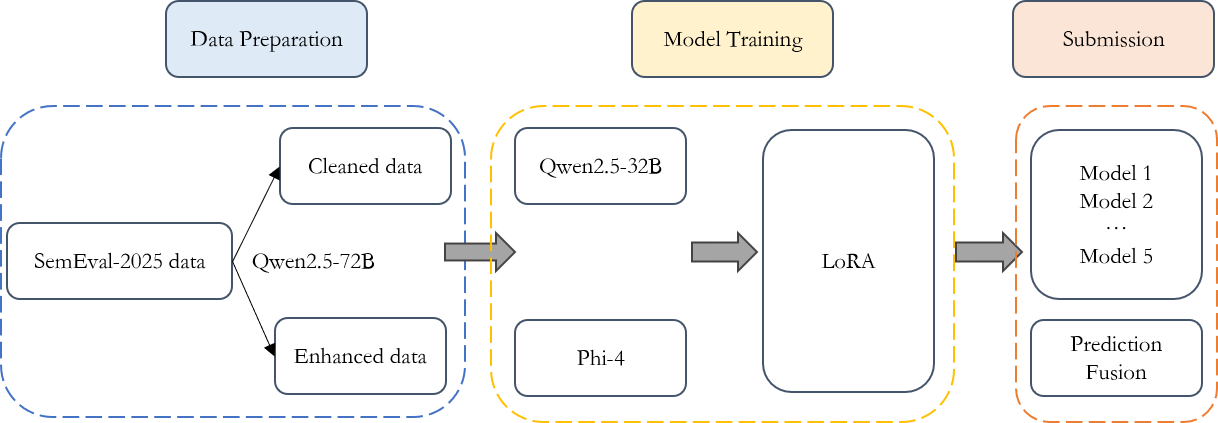
\includegraphics[width=0.95\textwidth]{figures/pateam_overview.png}
    \caption{System overview of the PATeam solution. Although Qwen2.5-32B is shown in the model training stage, all reported results were obtained with Phi-4 (taken directly from \cite{wan-etal-2025-pateam}).}
    \label{fig:pateam_overview}
\end{figure}
\end{comment}

\subsubsection{PATeam \cite{wan-etal-2025-pateam}}

Tento systém je pozoruhodný využitím jediného generatívneho LLM, ktorý rieši obe podúlohy spoločne vo forme viackolového dialógu, v kombinácii s bagging ensemble prístupom. V rámci predspracovania autori používajú regulárne výrazy na odstránenie nežiaducich webových artefaktov, ako sú hypertextové odkazy, HTML formátovanie a e-mailové adresy. Použité sú iba vstupné atribúty \textit{title} a \textit{text}.

V rámci augmentácie dát je LLM inštruovaný vygenerovať stručné zhrnutie každého vyčisteného textu, ktoré je následne spojené s pôvodným textom. Na rozdiel od ostatných spomenutých riešení tento prístup nevytvára nové vzorky, ale obohacuje existujúce. Podľa autorov zhrnutia pomáhajú štandardizovať zašumené texty a zvýrazniť informácie relevantné pre označenia produktu a hazardu. LLM použitý na tvorbu zhrnutí nie je v texte článku pomenovaný, avšak prehľad systému (obrázok~\ref{fig:pateam_overview}) naznačuje model Qwen2.5-72B. Na riešenie nevyváženosti tried je obohatený dataset následne oversamplovaný tak, aby každá trieda obsahovala aspoň päť vzoriek, pričom autori zistili, že táto hranica dosahuje na validačnej množine najlepšie výsledky.

Samotná predikcia je vykonávaná modelom Phi-4 doladeným pomocou LoRA \cite{hu2021lora}, ktorý formuluje obe podúlohy ako dialóg o dvoch kolách. V prvom kole model dostane nadpis, vyčistený text a vygenerované zhrnutie a predikuje kategóriu hazardu a kategóriu produktu (ST1). V druhom kole sú tieto predikcie pridané do promptu a model je požiadaný, aby určil konkrétnejší hazard a produkt (ST2). Týmto spôsobom všeobecnejšia predikcia usmerňuje tú detailnejšiu. Pre ensemble je použitý prístup bagging \cite{breiman1996bagging}: z trénovacích dát je vzorkovaním s opakovaním vytvorených päť podmnožín, na každej z nich je doladený samostatný model Phi-4 a finálna predikcia je získaná hlasovaním týchto piatich modelov (presná schéma hlasovania nie je uvedená).

Toto riešenie sa umiestnilo na štvrtom mieste v ST1 a na treťom mieste v ST2.

\begin{figure}
    \centering
    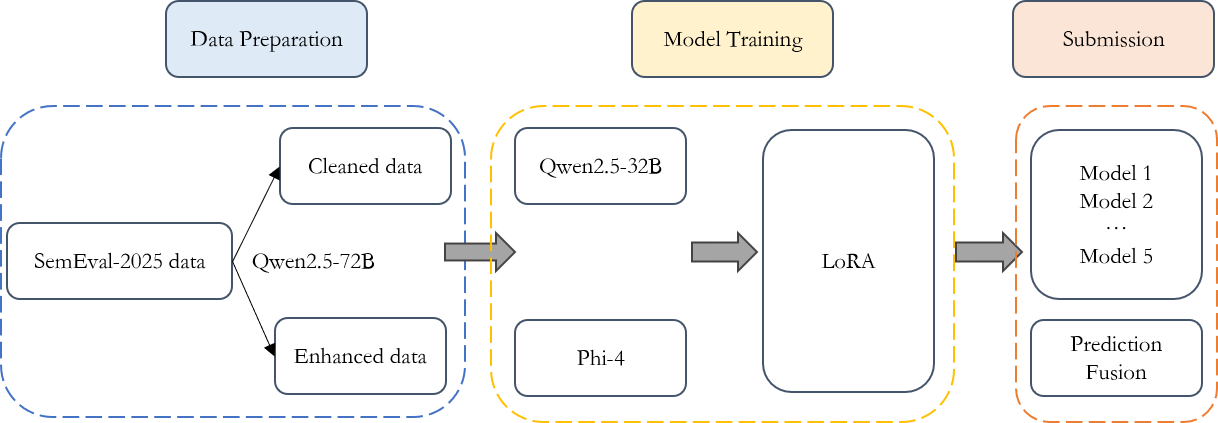
\includegraphics[width=0.95\textwidth]{figures/pateam_overview.png}
    \caption{Prehľad systému riešenia PATeam. Hoci je v štádiu trénovania modelu zobrazený model Qwen2.5-32B, všetky uvádzané výsledky boli získané s modelom Phi-4 (prevzaté priamo z \cite{wan-etal-2025-pateam}).}
    \label{fig:pateam_overview}
\end{figure}
\begin{comment}
\section{Vyhodnocovacie metriky a metodológia}

In order to evaluate our baseline solution, we will be using the same scoring process that was used for evaluating participant's submission in the challenge for both ST1 and ST2 \cite{randl-etal-2025-semeval}. The score is mainly based on macro F1, which was chosen due to the previously mentioned class imbalance inside of the dataset, ensuring that the score is not dominated by the most frequent labels. The following equations describe how the score for each task is calculated.

First the macro F1 score for hazard is computed using Equation~\ref{eq:macro_f1}. Here, $\mathrm{RCL}_i$ and $\mathrm{PRC}_i$ are the recall and precision of class $i$, and $n$ is the total number of classes.

\begin{equation}
  F_1(y, \hat{y}) = \frac{2}{n} \sum_{i=1}^{n} \frac{\mathrm{RCL}_i(y, \hat{y}) \cdot \mathrm{PRC}_i(y, \hat{y})}{\mathrm{RCL}_i(y, \hat{y}) + \mathrm{PRC}_i(y, \hat{y})}
  \label{eq:macro_f1}
\end{equation}

%Where $RCL_c$ is the recall and $PRC_c$ is the precision for a specific class $i$, with $n$ being the total number of classes. 

Then the dataset is filtered, keeping only the samples where the hazard was correctly predicted. This operation is mathematically described by Equation~\ref{eq:product_subset}. Here, $y^h$ and $y^p$ are the true hazard and product labels, $\hat{y}^h$ and $\hat{y}^p$ the predicted ones, and $m$ is the number of samples; $\hat{y}^{p|h}$ is defined analogously.

\begin{equation}
  y^{p|h} = \left\{ y^p_j \;\middle|\; \hat{y}^h_j = y^h_j \right\}, \quad j \in \{1, 2, \dots, m\}
  \label{eq:product_subset}
\end{equation}

Equation~\ref{eq:macro_f1} is then applied to the filtered dataset in order to produce the macro F1 score for product. The final task score is then calculated as the average of the macro F1 scores for the hazard and the product (Equation~\ref{eq:task_score}).

\begin{equation}
  S(Y, \hat{Y}) = \frac{F_1(y^h, \hat{y}^h) + F_1(y^{p|h}, \hat{y}^{p|h})}{2}
  \label{eq:task_score}
\end{equation}

The scoring process is done separately for ST1 and ST2. In ST1, the hazard and product categories are used, while ST2 uses the exact hazard and product.

\subsection{Metodológia}

The main focus of the baseline will be the creation of a reproducible solution that incorporates features of the previously highlighted systems while still remaining lightweight, so that it can be potentially expanded upon in the second part of this project. The resulting score of this solution will then be compared against the systems which form the official ranking, to see which place it would obtain for each sub-task.

For our baseline solution we will be using the official dataset published on Zenodo \cite{randl_2025_15007331}, while also using the official train/validation/test splits provided by the organizers of the challenge. The sizes of these subsets are:

\begin{itemize}
    \item Training -- 5 082 ($\sim$76,5\%)
    \item Validation -- 565 ($\sim$8,5\%)
    \item Test -- 997 ($\sim$15,0\%)
\end{itemize}
\end{comment}

\section{Vyhodnocovacie metriky a metodológia}

Na vyhodnotenie nášho baseline riešenia bude použitý rovnaký proces hodnotenia, aký bol v súťaži použitý na vyhodnotenie riešení odovzdaných účastníkmi, a to pre ST1 aj ST2 \cite{randl-etal-2025-semeval}. Skóre je založené predovšetkým na metrike macro F1, ktorá bola zvolená z dôvodu už spomenutej nevyváženosti tried v datasete, čím je zabezpečené, že skóre nie je ovplyvňované najmä najfrekventovanejšími označeniami (labels). Nasledujúce rovnice opisujú, ako je vypočítané skóre pre každú z podúloh.

Najprv je pomocou rovnice~\ref{eq:macro_f1} vypočítané skóre macro F1 pre hazard. Tu $\mathrm{RCL}_i$ a $\mathrm{PRC}_i$ predstavujú recall a precision triedy $i$ a $n$ je celkový počet tried.

\begin{equation}
  F_1(y, \hat{y}) = \frac{2}{n} \sum_{i=1}^{n} \frac{\mathrm{RCL}_i(y, \hat{y}) \cdot \mathrm{PRC}_i(y, \hat{y})}{\mathrm{RCL}_i(y, \hat{y}) + \mathrm{PRC}_i(y, \hat{y})}
  \label{eq:macro_f1}
\end{equation}

%Kde $RCL_c$ je recall a $PRC_c$ je precision pre konkrétnu triedu $i$, pričom $n$ je celkový počet tried.

Následne je dataset prefiltrovaný, pričom sú ponechané iba vzorky, pri ktorých bol hazard predikovaný správne. Táto operácia je matematicky opísaná rovnicou~\ref{eq:product_subset}. Tu $y^h$ a $y^p$ predstavujú skutočné označenia hazardu a produktu, $\hat{y}^h$ a $\hat{y}^p$ predikované označenia a $m$ je počet vzoriek. $\hat{y}^{p|h}$ je definované analogicky.

\begin{equation}
  y^{p|h} = \left\{ y^p_j \;\middle|\; \hat{y}^h_j = y^h_j \right\}, \quad j \in \{1, 2, \dots, m\}
  \label{eq:product_subset}
\end{equation}

Na prefiltrovaný dataset je následne aplikovaná rovnica~\ref{eq:macro_f1}, čím je získané skóre macro F1 pre produkt. Výsledné skóre úlohy je potom vypočítané ako priemer skóre macro F1 pre hazard a produkt (rovnica~\ref{eq:task_score}).

\begin{equation}
  S(Y, \hat{Y}) = \frac{F_1(y^h, \hat{y}^h) + F_1(y^{p|h}, \hat{y}^{p|h})}{2}
  \label{eq:task_score}
\end{equation}

Proces hodnotenia je vykonávaný samostatne pre ST1 a ST2. V ST1 sú použité kategórie hazardu a produktu, zatiaľ čo v ST2 sú použité konkrétne hazardy a produkty.

\subsection{Metodológia}

Hlavným cieľom baseline riešenia bude vytvorenie reprodukovateľného riešenia, ktoré bude zahŕňať prvky spomenutých systémov a zároveň zostane výpočtovo nenáročné, aby ho bolo možné v druhej časti tohto projektu ďalej rozšíriť. Výsledné skóre tohto riešenia bude následne porovnané so ostatnými referenčnými riešeniami a taktiež systémami, ktoré tvoria oficiálny rebríček, aby bolo možné určiť, na ktorom mieste by sa v jednotlivých podúlohách umiestnilo.

Pre naše baseline riešenie bude použitý oficiálny dataset zverejnený na platforme Zenodo \cite{randl_2025_15007331}, pričom budú použité aj oficiálne rozdelenia na trénovaciu, validačnú a testovaciu množinu poskytnuté organizátormi súťaže. Veľkosti týchto podmnožín sú:

\begin{itemize}
    \item Trénovacia množina -- 5\,082 ($\sim$76,5~\%)
    \item Validačná množina -- 565 ($\sim$8,5~\%)
    \item Testovacia množina -- 997 ($\sim$15,0~\%)
\end{itemize}
\begin{comment}
\section{Návrh a implementácia baseline riešenia}

In this chapter the design and implementation process of the baseline will be detailed. The design subsection will give a broad overview of the system architecture and explain why certain parts were chosen, while the implementation subsection will concretely detail each process used as part of the pipeline.

\subsection{Návrh baseline riešenia}

In order to help explain our reasoning for the design of the system, the following list broadly describes the general trends found in each examined system with each point being present in at least two of the solutions. 

\begin{itemize}
    \item Text concatenation of input features + text cleaning (SRCB, Anastasia, PATeam) 
    \item Usage of data augmentation (All examined solutions)
    \item Usage of LLMs for data augmentation (SRCB, MyMy, PATeam)
    \item Usage of BERT architecture for at least partial classification (SRCB, Anastasia, MyMy)
    \item Usage of fine-tuned LLMs for classification (SRCB, MyMy, PATeam)
    \item Ensemble strategies (All examined solutions)
\end{itemize}

With that in mind, our team decided that our baseline would essentially be a simplified version of the SRCB solution with three key changes:

\begin{enumerate}
    \item Data augmentation would be done with EDA \cite{wei2019eda}, not with the help of an LLM. While the team did consider using an LLM for this purpose, it was ultimately decided that it would be too advanced for a baseline solution due to the complexity, time and the subsequent costs associated with using an LLM this way.
    
    \item For training the BERT model, focal loss \cite{lin2017focal} would be used, specifically the binary variant (due to the one-vs-all setup). This is an idea borrowed from Anastasia, where the authors claim it can help with imbalanced datasets. Since EDA generally produces less diverse samples than LLM-based generation, more of the burden of handling the class imbalance falls on the loss function, which is why focal loss could prove advantageous.   
    
    \item The LLM used for the final prediction would neither be fine-tuned nor use SRCB’s label attention module, instead it would simply be given a multiple-choice prompt with the reduced label set from the BERT model.
\end{enumerate}

While this solution only effectively uses three out of the six mentioned trends, it was decided this would be a good lightweight starting point that could potentially be easily expanded to include more of the aforementioned trends. See Figure~\ref{fig:placeholder} for an overview of the proposed pipeline.
 
\begin{figure}
    \centering
    
\includegraphics[width=0.35\textwidth]{figures/floppa_placeholder.jpg}
    \caption{Placeholder}
    \label{fig:placeholder}
\end{figure}
\end{comment}

\section{Návrh a implementácia baseline riešenia}

V tejto kapitole bude podrobne opísaný proces návrhu a implementácie baseline riešenia. Podkapitola o návrhu poskytne všeobecný prehľad architektúry systému a vysvetlí, prečo boli zvolené jednotlivé časti, zatiaľ čo podkapitola o implementácii konkrétne opíše každý proces, ktorý je súčasťou pipeline.

\subsection{Návrh baseline riešenia}

Na objasnenie úvah, ktoré viedli k návrhu systému, slúži nasledujúci zoznam, ktorý všeobecne opisuje trendy nájdené v preskúmaných systémoch, pričom každý bod sa vyskytuje aspoň v dvoch riešeniach.

\begin{itemize}
    \item Spojenie vstupných atribútov do jedného textu + čistenie textu (SRCB, Anastasia, PATeam)
    \item Využitie augmentácie dát (všetky preskúmané riešenia)
    \item Využitie LLM na augmentáciu dát (SRCB, MyMy, PATeam)
    \item Využitie architektúry BERT aspoň na čiastočnú klasifikáciu (SRCB, Anastasia, MyMy)
    \item Využitie doladených LLM na klasifikáciu (SRCB, MyMy, PATeam)
    \item Ensemble stratégie (všetky skúmané riešenia)
\end{itemize}

S ohľadom na tieto trendy sa náš tím rozhodol, že baseline riešenie bude v podstate zjednodušenou verziou riešenia SRCB s tromi kľúčovými zmenami:

\begin{enumerate}
    \item Augmentácia dát bude vykonaná pomocou metódy EDA \cite{wei2019eda}, nie pomocou LLM. Hoci tím zvažoval využitie LLM na tento účel, nakoniec bolo rozhodnuté, že by to bolo pre baseline riešenie príliš pokročilé z dôvodu zložitosti, časovej náročnosti a s tým spojených nákladov na takéto využitie LLM.
    
    \item Pri trénovaní modelu BERT bude použitá stratová funkcia focal loss \cite{lin2017focal}, konkrétne jej binárna varianta (z dôvodu použitia prístupu one-vs-all). Ide o myšlienku prevzatú z riešenia Anastasia, ktorého autori tvrdia, že táto funkcia môže pomôcť pri nevyvážených datasetoch. Keďže EDA vo všeobecnosti vytvára menej rozmanité vzorky ako generovanie pomocou LLM, väčšia časť zodpovednosti za riešenie nevyváženosti tried pripadá na stratovú funkciu, a preto by sa focal loss mohla ukázať ako výhodná.
    
    \item LLM použitý na finálnu predikciu nebude doladený ani nebude využívať modul label attention z riešenia SRCB. Namiesto toho mu bude jednoducho poskytnutý prompt s výberom z viacerých možností, ktorý obsahuje zúženú množinu označení z modelu BERT.
\end{enumerate}

Hoci toto riešenie v skutočnosti využíva iba tri zo šiestich spomenutých trendov, bolo rozhodnuté, že bude vhodným a výpočtovo nenáročným začiatočným bodom, ktorý by mohol byť potenciálne jednoducho rozšírený o ďalšie zo spomenutých trendov. Pre prehľad navrhutej pipeline viď obrázok~\ref{fig:baseline_architecture}.
 
\begin{figure}
    \centering
    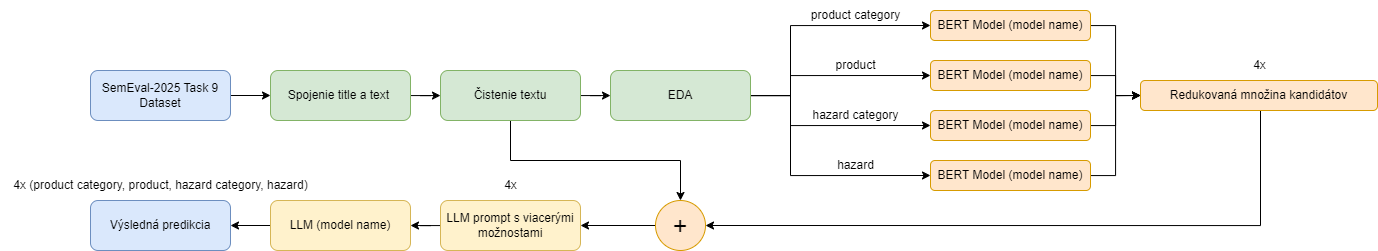
\includegraphics[width=1\textwidth]{figures/baseline_pipeline.drawio.png}
    \caption{Pipeline navrhnutého baseline riešenia.}
    \label{fig:baseline_architecture}
\end{figure}

\begin{comment}
\subsection{Implementácia baseline riešenia}

This subsection describes the individual steps of the baseline pipeline in the order in which they are performed: data preparation, data augmentation, candidate recall, LLM prediction and evaluation.

\subsubsection{Príprava dát}

As the first step, the \textit{title} and \textit{text} features of each sample are concatenated into a single text, while the remaining features (year, month, day and country) are not used. Following the SRCB solution, the resulting texts are then cleaned by normalising whitespace and line breaks, removing duplicate segments and converting all characters to lowercase. In line with SRCB, each of the four target labels (hazard category and product category for ST1, exact hazard and exact product for ST2) is treated as a separate classification problem.

\subsubsection{Augmentácia dát}

To address the class imbalance, the training set is augmented using EDA \cite{wei2019eda}. The augmentation is performed only after the data has been split, and only on the training set, to ensure that no synthetic samples end up in the validation or test sets.

Instead of augmenting the data separately for each classification problem, a single augmented dataset is created and shared by all four classifiers, with every augmented sample keeping all four labels of the sample it was created from. Since the exact product label contains by far the most underrepresented classes, it is used to drive the augmentation: every product class with fewer than (target sample count) training samples is filled up to this count by creating EDA variants of its existing samples. As each augmented sample also carries the remaining three labels, this indirectly increases their representation as well.

Each variant is created by applying the four EDA operations, namely synonym replacement, random insertion, random swap and random deletion, with (change rate) of the words in the text being modified. Since the exact hazards and products often appear literally in the text, the words corresponding to the sample's labels are protected from modification, and the \textit{title} is left unchanged, with EDA applied only to the \textit{text}. The augmentation is implemented using (EDA implementation) with a fixed random seed (seed). In total, (number of augmented samples) synthetic samples were added to the training set, increasing its size from 5\,082 to (augmented training set size) samples.

\subsubsection{Modul výberu kandidátov}

The candidate recall module reduces the set of possible labels before the final prediction by the LLM. For this purpose, (BERT model) is fine-tuned separately for each of the four classification problems, resulting in four models. Following SRCB, a one-vs-all approach is used, implemented as a multi-label classification head with one sigmoid output per label on top of the shared encoder, so that each output acts as a binary classifier for its respective label.

The models are trained using the binary variant of focal loss \cite{lin2017focal} with the parameters $\gamma$ = ($\gamma$) and $\alpha$ = ($\alpha$). The training uses the AdamW optimizer with a learning rate of (learning rate), a batch size of (batch size) and a maximum input length of (maximum length) tokens, for at most (number of epochs) epochs with early stopping based on the validation set.

After training, all labels with a predicted probability above (probability threshold) are selected as candidates. If no label exceeds this threshold, the (top-k) labels with the highest probability are selected instead, and the number of candidates is limited to at most (maximum number of candidates) in order to keep the prompts for the following step short. The resulting candidate recall, i.e.\ the proportion of samples whose correct label is among the selected candidates, was (candidate recall) on the validation set.

\subsubsection{Predikcia pomocou LLM}

The final prediction is made by an off-the-shelf LLM, (LLM), without any fine-tuning. For each sample and classification problem, a multiple-choice prompt is constructed containing a short task description, the cleaned title and text of the sample, and the candidate labels from the previous step as a numbered list, together with an instruction to answer with exactly one of the listed labels and nothing else. For ST1, (all labels / the candidate labels) are included in the prompt, since the number of categories in this sub-task is small. The candidate labels are ordered by their predicted probability from the candidate recall module, with the most probable label listed first. The full format of the prompt  is shown in Figure~\ref{fig:baseline_prompt}.

\begin{figure}
    \centering
    
\includegraphics[width=0.25\textwidth]{figures/floppa_placeholder.jpg}
    \caption{LLM prompt used to determine the final predicted lable.}
    \label{fig:baseline_prompt}
\end{figure}

To obtain deterministic outputs, the temperature is set to (temperature). The LLM's answers are then mapped to the label set: if the answer exactly matches one of the candidate labels, that label is used; otherwise, the most similar label is selected using (string matching method). If no sufficiently similar label is found, the candidate with the highest probability from the candidate recall module is used as a fallback.
\end{comment}

\subsection{Implementácia baseline riešenia}

Táto podkapitola opisuje jednotlivé kroky pipeline baseline riešenia v poradí, v akom sú vykonávané: príprava dát, augmentácia dát, výber kandidátov, a výsledná predikcia pomocou LLM.

\subsubsection{Príprava dát}

V prvom kroku sú atribúty \textit{title} a \textit{text} každej vzorky spojené do jedného textu, pričom zvyšné atribúty (\textit{year}, \textit{month}, \textit{day} a \textit{country}) nie sú použité. Podľa vzoru riešenia SRCB sú výsledné texty následne vyčistené normalizáciou bielych znakov a zalomení riadkov, odstránením duplicitných úsekov a prevodom všetkých znakov na malé písmená. V súlade s riešením SRCB je každé zo štyroch cieľových označení (kategória hazardu a kategória produktu pre ST1, konkrétny hazard a konkrétny produkt pre ST2) považované za samostatný klasifikačný problém.

\subsubsection{Augmentácia dát}

Na riešenie nevyváženosti tried je trénovacia množina augmentovaná pomocou metódy EDA \cite{wei2019eda}. Augmentácia je vykonaná až po rozdelení dát a iba na trénovacej množine, aby sa zabezpečilo, že sa žiadne syntetické vzorky nedostanú do validačnej ani testovacej množiny.

Namiesto samostatnej augmentácie dát pre každý klasifikačný problém je vytvorený jeden augmentovaný dataset, ktorý je zdieľaný všetkými štyrmi klasifikátormi, pričom každá augmentovaná vzorka si zachováva všetky štyri označenia vzorky, z ktorej bola vytvorená. Keďže označenie konkrétneho produktu obsahuje zďaleka najviac málo zastúpených tried, augmentácia je riadená práve ním: každá trieda produktu s menej ako (target sample count) trénovacími vzorkami je doplnená na tento počet vytvorením EDA variantov jej existujúcich vzoriek. Keďže každá augmentovaná vzorka nesie aj zvyšné tri označenia, nepriamo sa tým zvyšuje aj ich zastúpenie.

Každý variant je vytvorený aplikovaním štyroch operácií EDA, konkrétne nahradenia synonymom, náhodného vloženia, náhodnej zámeny a náhodného vymazania, pričom je upravených (change rate) slov v texte. Keďže konkrétne hazardy a produkty sa v texte často vyskytujú doslovne, slová zodpovedajúce označeniam vzorky sú chránené pred úpravou a \textit{title} zostáva nezmenený, pričom EDA je aplikovaná iba na \textit{text}. Augmentácia je implementovaná pomocou (EDA implementation) s pevne nastaveným náhodným seedom (seed). Celkovo bolo do trénovacej množiny pridaných (number of augmented samples) syntetických vzoriek, čím sa jej veľkosť zvýšila z 5\,082 na (augmented training set size) vzoriek.

\subsubsection{Modul výberu kandidátov}

Modul výberu kandidátov zužuje množinu možných označení pred finálnou predikciou pomocou LLM. Na tento účel je model (BERT model) doladený samostatne pre každý zo štyroch klasifikačných problémov, výsledkom čoho sú štyri modely. Podľa vzoru riešenia SRCB je použitý prístup one-vs-all, implementovaný ako multi-label klasifikačná hlava s jedným sigmoidovým výstupom pre každé označenie nad zdieľaným enkodérom, takže každý výstup funguje ako binárny klasifikátor pre príslušné označenie.

Modely sú trénované pomocou binárnej varianty focal loss \cite{lin2017focal} s parametrami $\gamma$ = ($\gamma$) a $\alpha$ = ($\alpha$). Trénovanie využíva optimalizátor AdamW s rýchlosťou učenia (learning rate), veľkosťou dávky (batch size) a maximálnou dĺžkou vstupu (maximum length) tokenov, pričom trvá najviac (number of epochs) epoch s predčasným zastavením (early stopping) na základe validačnej množiny.

Po natrénovaní sú ako kandidáti vybrané všetky označenia s predikovanou pravdepodobnosťou vyššou ako (probability threshold). Ak žiadne označenie túto hranicu neprekročí, namiesto toho je vybraných (top-k) označení s najvyššou pravdepodobnosťou, pričom počet kandidátov je obmedzený na najviac (maximum number of candidates), aby prompty pre nasledujúci krok zostali krátke. Výsledný recall kandidátov, t.\,j. podiel vzoriek, ktorých správne označenie sa nachádza medzi vybranými kandidátmi, dosiahol na validačnej množine hodnotu (candidate recall).

\subsubsection{Predikcia pomocou LLM}

Finálna predikcia je vykonaná bežne dostupným LLM (LLM) bez akéhokoľvek doladenia. Pre každú vzorku a klasifikačný problém je zostavený prompt s výberom z viacerých možností, ktorý obsahuje krátky opis úlohy, vyčistený nadpis a text vzorky a kandidátske označenia z predchádzajúceho kroku vo forme číslovaného zoznamu, spolu s inštrukciou odpovedať práve jedným z uvedených označení a ničím iným. Pre ST1 sú v prompte zahrnuté (all labels / the candidate labels), keďže počet kategórií v tejto podúlohe je malý. Kandidátske označenia sú zoradené podľa predikovanej pravdepodobnosti z modulu výberu kandidátov, pričom najpravdepodobnejšie označenie je uvedené ako prvé. Úplný formát promptu je zobrazený na obrázku~\ref{fig:baseline_prompt}.

\begin{figure}
    \centering
    
\includegraphics[width=0.25\textwidth]{figures/floppa_placeholder.jpg}
    \caption{Prompt pre LLM použitý na určenie výsledného predikovaného označenia.}
    \label{fig:baseline_prompt}
\end{figure}

Na získanie deterministických výstupov je teplota nastavená na (temperature). Odpovede LLM sú následne priradené k množine označení: ak sa odpoveď presne zhoduje s jedným z kandidátskych označení, je použité toto označenie, v opačnom prípade je pomocou (string matching method) vybrané najpodobnejšie označenie. Ak nie je nájdené dostatočne podobné označenie, ako záložné riešenie je použitý kandidát s najvyššou pravdepodobnosťou z modulu výberu kandidátov.

\begin{comment}
\section{Výsledky baseline riešenia}

Our solution achieved a (score) placing us (ST1 placement) for ST1 and (score) placing us (ST2 placement) for ST2. See Figure~\ref{fig:baseline_cm} for the resulting confusion matrices.

\begin{figure}
    \centering
    
\includegraphics[width=0.25\textwidth]{figures/floppa_placeholder.jpg}
    \caption{Confusion matrices using our baseline for ST1 and ST2}
    \label{fig:baseline_cm}
\end{figure}

\section{Použitie agentov a LLM mimo riešenia}

A LLM specifically Claude Opus 5.5 was used during the development of this project for:

\begin{itemize}
    \item Text critique (e.q. "Here is my section on MyMy, what do you think ? Is there anything that should be added ?")
    \item Clarification of concepts (e,q "Was the pipeline for both subtasks the same ?", "How is the sample and relevant documents combined into a prompt, are they just attached or are they somehow embedded together ?")
    \item Image extraction from documents (e.q "Can you extract the LLM prediction module image from page 999 for me ?")
    \item Language translation
\end{itemize}
\end{comment}

\section{Výsledky baseline riešenia}

Naše riešenie dosiahlo v ST1 skóre (score), čím sa umiestnilo na (ST1 placement) mieste, a v ST2 skóre (score), čím sa umiestnilo na (ST2 placement) mieste. Pre výsledné konfúzné matice pre ST1 viď obrázok~\ref{fig:baseline_cm_product},~\ref{fig:baseline_cm_hazard} (ST2 má príliš veľa možných označení pre zmysluplnú vizualizáciu).

\begin{figure}
    \centering
    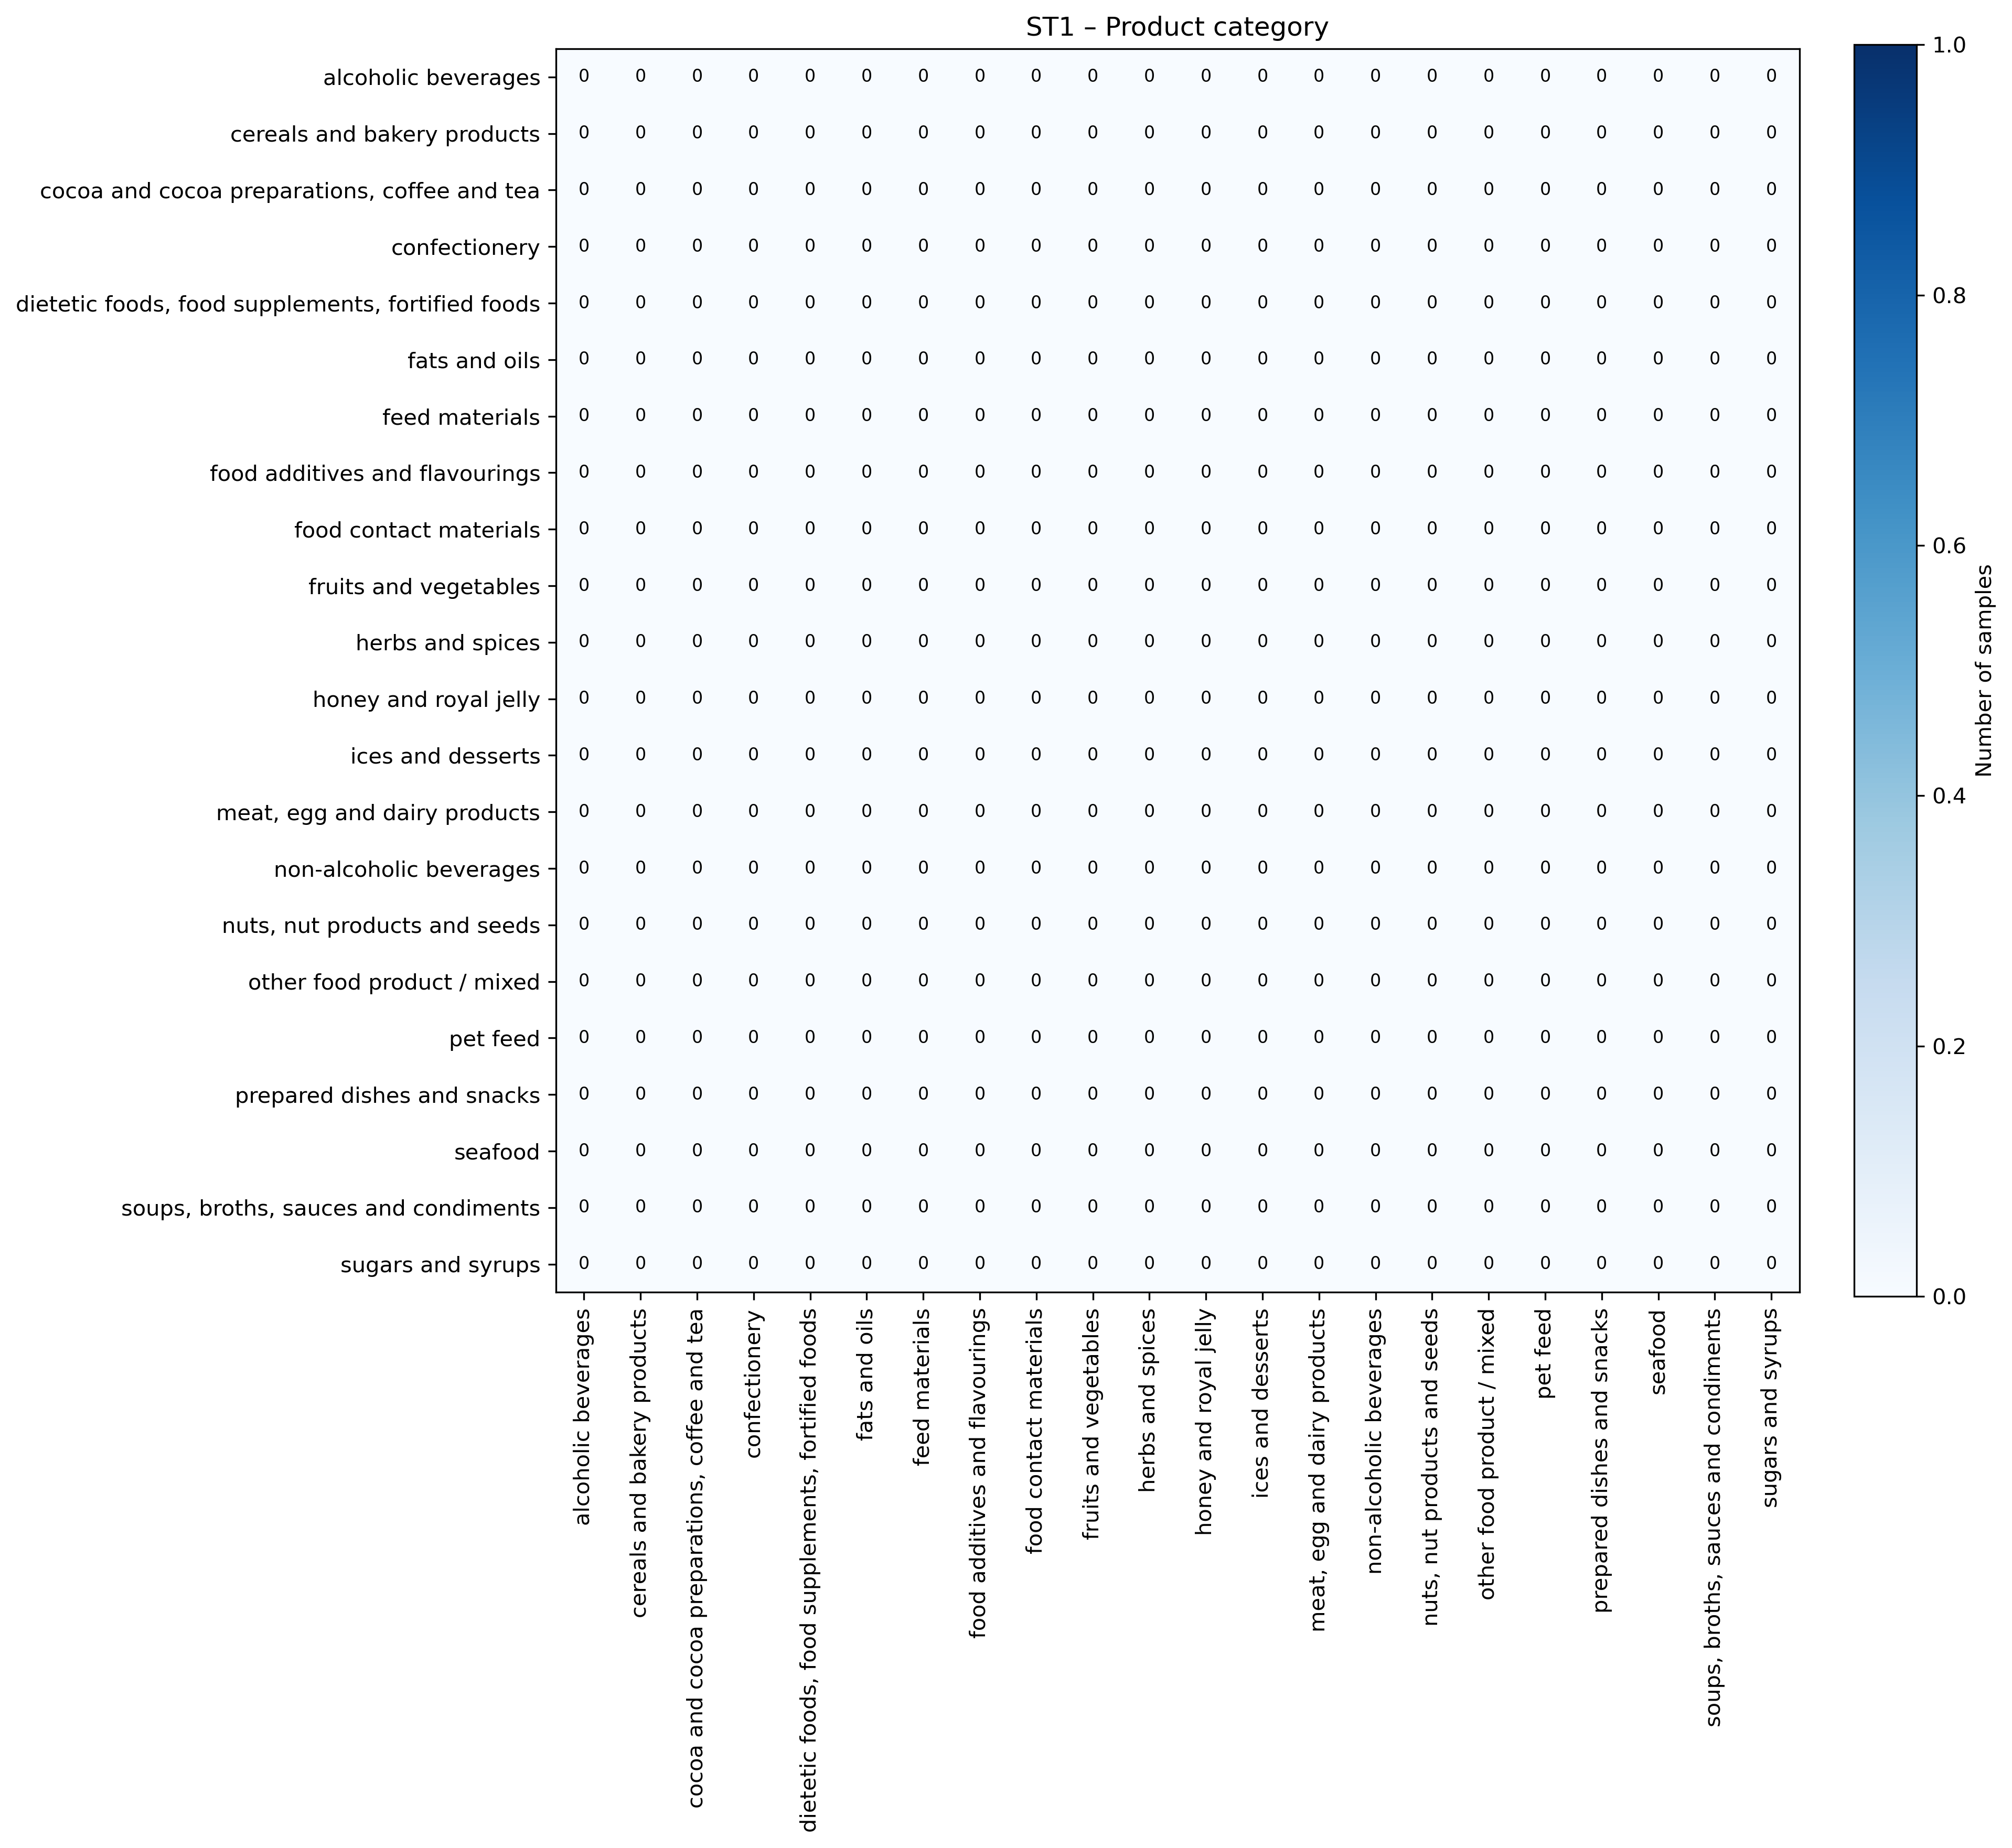
\includegraphics[width=0.95\textwidth]{figures/st1_confusion_product.png}
    \caption{Konfúzna matica pre baseline riešenie pre ST1 - product.}
    \label{fig:baseline_cm_product}
\end{figure}

\begin{figure}
    \centering
    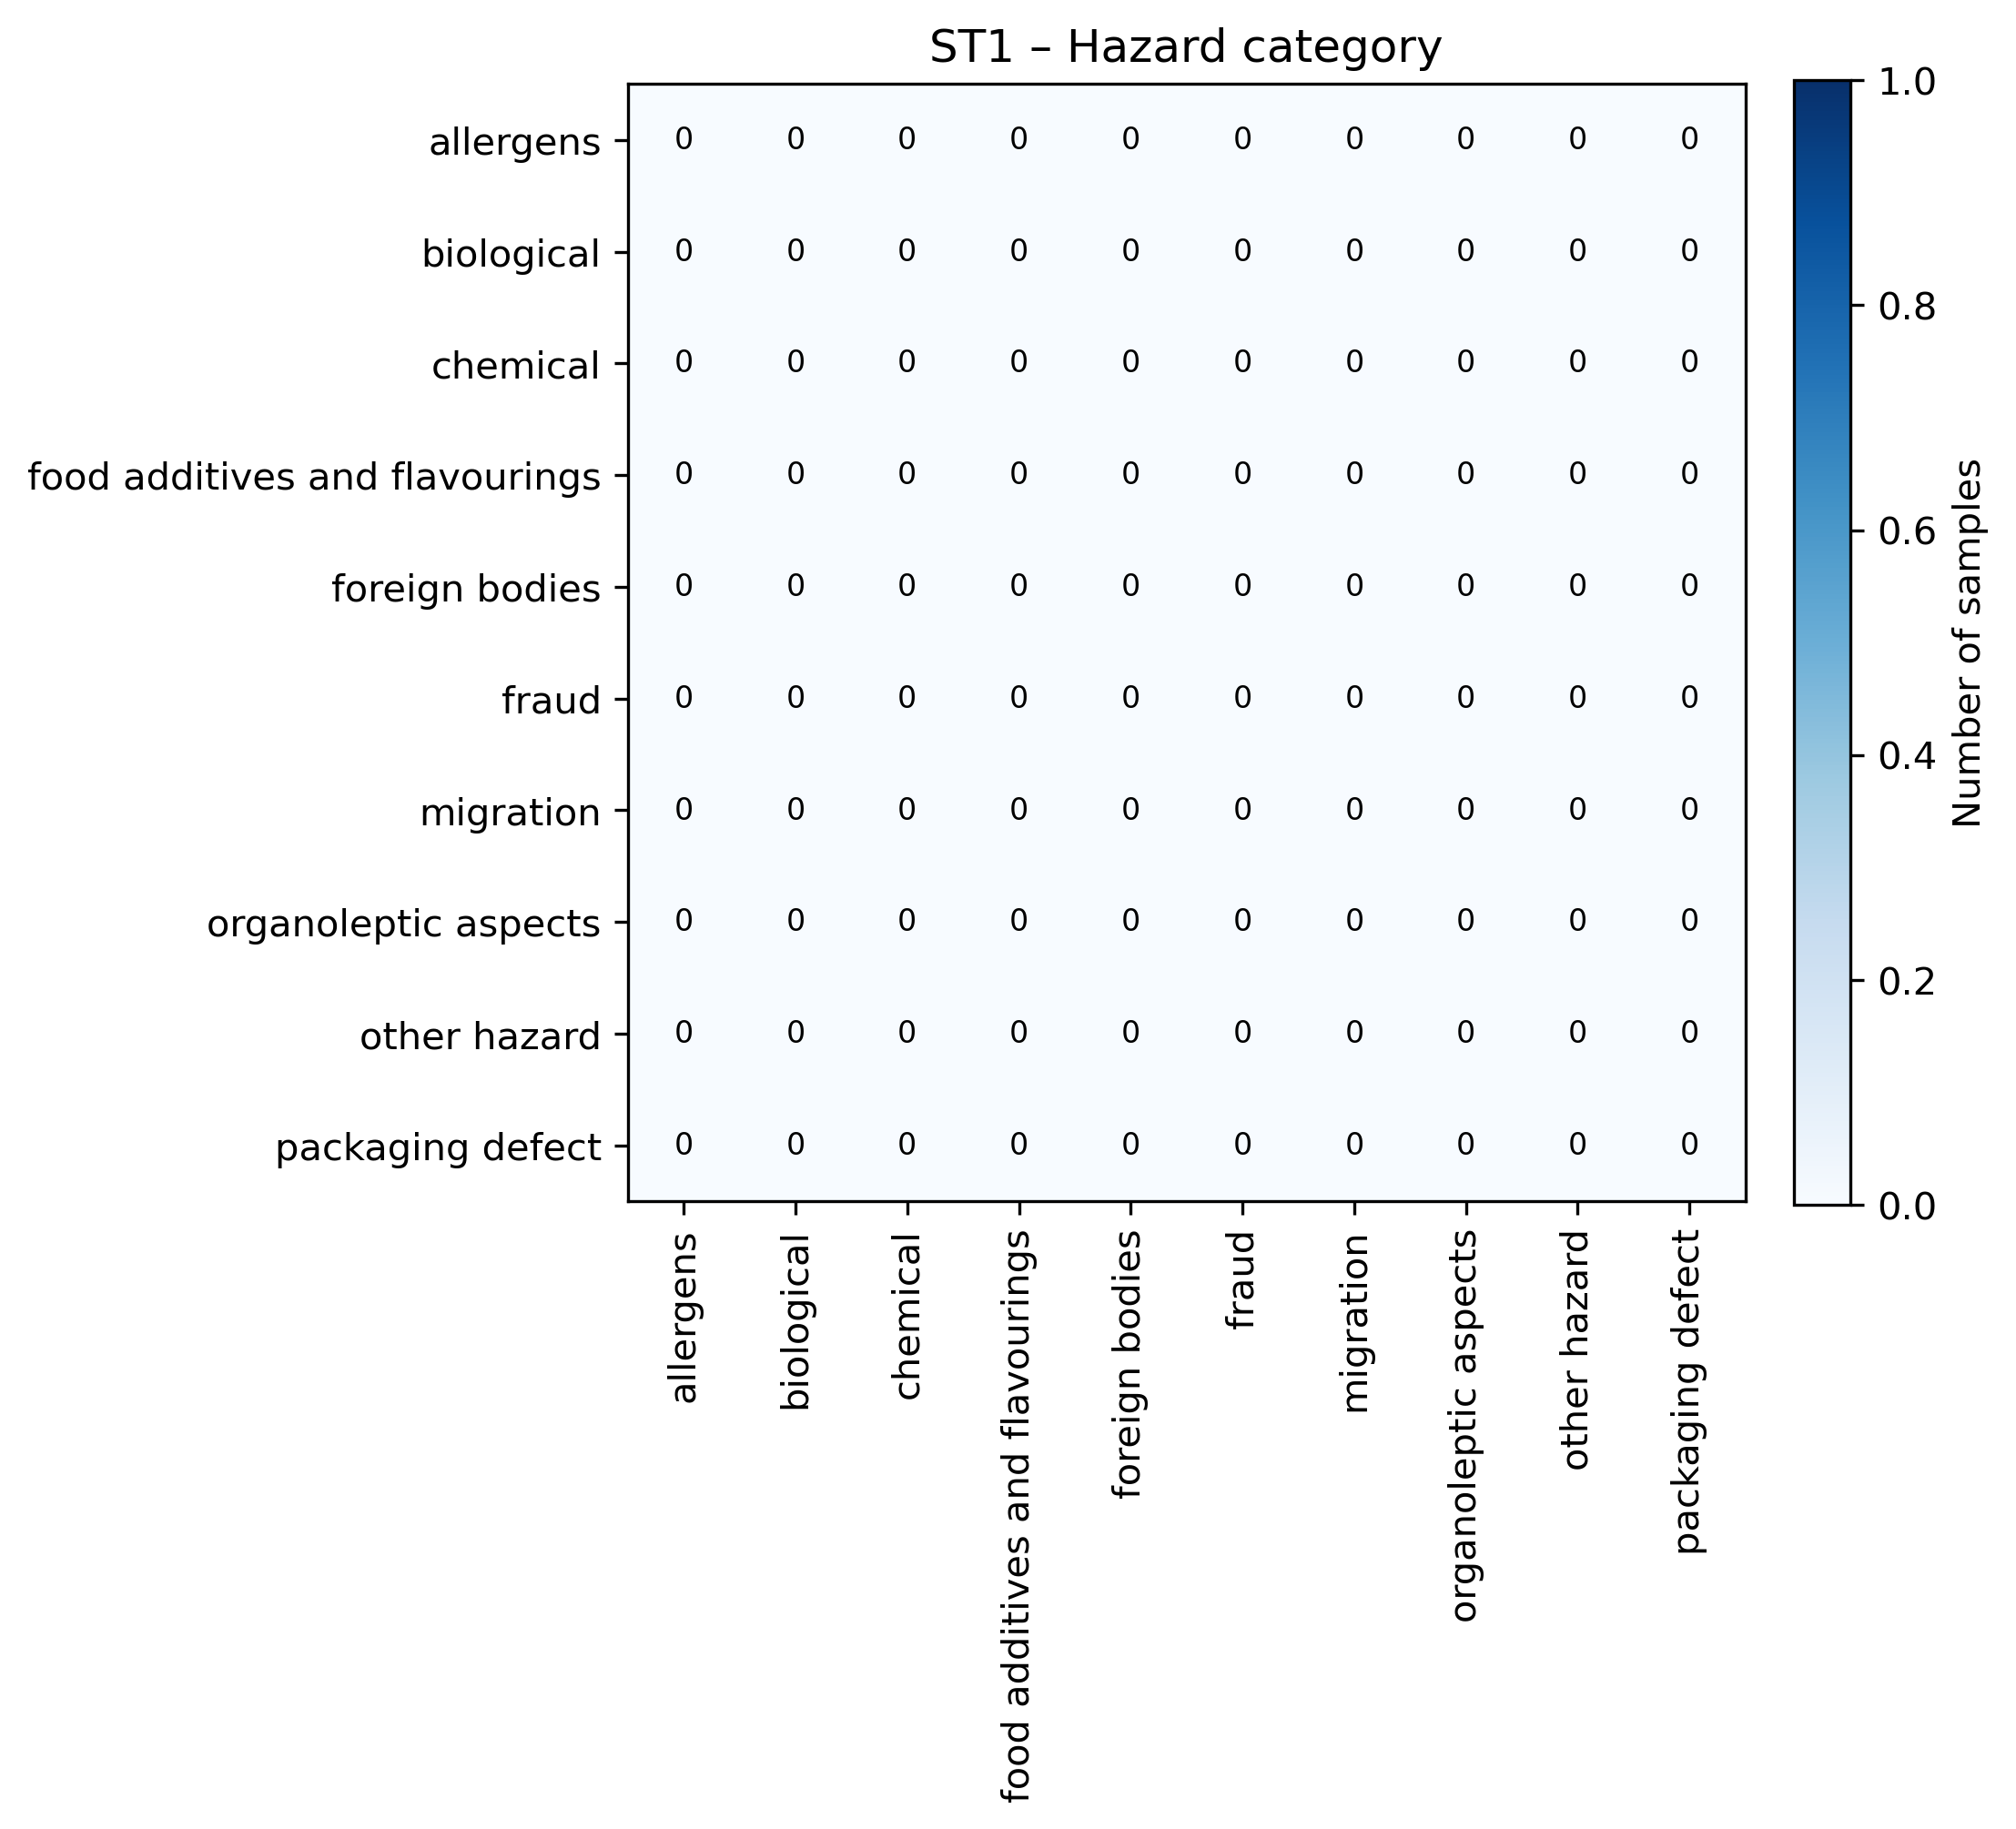
\includegraphics[width=0.95\textwidth]{figures/st1_confusion_hazard.png}
    \caption{Konfúzna matica pre baseline riešenie pre ST1 - hazard.}
    \label{fig:baseline_cm_hazard}
\end{figure}

\section{Použitie agentov a LLM mimo riešenia}

Počas vývoja tohto projektu bol použitý LLM, konkrétne Claude Opus 5.5, na:

\begin{itemize}
    \item Kritiku textu (napr. \uv{Here is my section on MyMy, what do you think? Is there anything that should be added?})
    \item Objasnenie pojmov (napr. \uv{Was the pipeline for both subtasks the same?}, \uv{How is the sample and relevant documents combined into a prompt, are they just attached or are they somehow embedded together?})
    \item Extrakciu obrázkov z dokumentov (napr. \uv{Can you extract the LLM prediction module image from page 999 for me?})
    \item Preklad textu
\end{itemize}

\bibliographystyle{unsrt}
\bibliography{references}

\end{document}